\documentclass[11pt,a4paper,oneside]{report}
\usepackage[utf8]{inputenc}
\usepackage{polski}
\usepackage[polish]{babel}
\usepackage{indentfirst}
\usepackage{url}

\usepackage{appendix}
\usepackage{multirow}
\usepackage{booktabs}
\usepackage{array}

\usepackage{amsmath}
\usepackage{color}
\usepackage{listings}
\usepackage{graphicx}
\usepackage{hyperref}

%\newcommand{\bib}[1]{\cite{#1}

% marginesy
\textwidth\paperwidth
\advance\textwidth -55mm
\oddsidemargin-0.9in
\advance\oddsidemargin 33mm
\evensidemargin-0.9in
\advance\evensidemargin 33mm
\topmargin -1in
\advance\topmargin 25mm
\setlength\textheight{48\baselineskip}
\addtolength\textheight{\topskip}
\marginparwidth 15mm

%\lstlistoflistings
\definecolor{darkgray}{rgb}{0.95,0.95,0.95}
\definecolor{dkgreen}{rgb}{0,0.6,0}
\definecolor{mauve}{rgb}{0.58,0,0.82}

\lstset{language=C}
\lstset{basicstyle=\footnotesize}
\lstset{backgroundcolor=\color{darkgray}}
\lstset{numbers=left, numberstyle=\tiny, stepnumber=2, numbersep=5pt}
\lstset{keywordstyle=\color{red}\bfseries\emph}
\lstset{commentstyle=\color{dkgreen}}
\lstset{stringstyle=\color{mauve}}

\linespread{1.2}

\begin{document}
%\title{ Pomiar opóźnienia ramek standardu 802.11 - narzędzie \emph{hop-sniffer}. }
%\author{ Marcin Harasimczuk }
%\maketitle

\thispagestyle{empty}

\begin{flushright}
 \begin{tabular}{c}
  Rok akademicki 2011/2012
 \end{tabular}
\end{flushright}

\begin{flushleft}
 \begin{tabular}{c}
  Politechnika Warszawska \\
  Wydział Elektroniki i Technik Informacyjnych \\
  Instytut Informatyki
 \end{tabular}
\end{flushleft}

\vspace{24pt}

\begin{center}
 
\includegraphics[width=0.3\textwidth]{img/pw_logo.pdf}
\end{center}

\vspace{12pt}

\begin{center}
 {\Large PRACA DYPLOMOWA INŻYNIERSKA}\\
 \vspace{24pt}
 {\large Marcin Harasimczuk}\\
 \vspace{24pt}
 {\LARGE Pomiar opóźnienia ramek standardu \emph{802.11}- narzędzie \emph{hop-sniffer}.}\\
\end{center}

\vfill

\begin{flushright}
 \begin{tabular}{c}
  Opiekun pracy \\
  dr inż. Jacek Wytrębowicz
 \end{tabular}
\end{flushright}

\vspace{12pt}

\begin{flushleft}
 \begin{tabular}{c}
  Ocena:\dotfill \\ \addlinespace[18pt]
  \dotfill \\
  Podpis Przewodniczącego \\
  Komisji Egzaminu Dyplomowego
 \end{tabular}
\end{flushleft}

\thispagestyle{empty}

\begin{tabular}{@{}c c}
  \multirow{4}{*}{
\includegraphics{img/zdjecie.pdf}} & \\
  & Specjalność: \hfill Inżynieria Systemów Informatycznych \\
\addlinespace[24pt]
  & Data urodzenia: \hfill 1988.01.28 \\ \addlinespace[24pt]
  & Data rozpoczęcia studiów: \hfill 2008.02.21
\end{tabular}

\vspace{48pt}

Życiorys.
\vfill

Urodziłem się 28 stycznia 1988 w Łodzi. Od 2004 roku uczęszczałem do L LO im. Ruy Barbosy w Warszawie. W 2007 roku ukończyłem szkołę średnią. Od lutego 2008 roku podjąłem studia na Wydziale Elektroniki i Technik Informacyjnych Politechniki Warszawskiej na kierunku Informatyka i specjalności Inżynieria Systemów Informatycznych.

Po uzyskaniu tytułu inżyniera chcę podjąć studia drugiego stopnia na wydziale Elektroniki i Technik Informacyjnych Politechniki Warszawskiej. W obszarze moich zainteresowań naukowych leżą systemy wbudowane i mikroprocesorowe, programowanie niskopoziomowe i zagadnienia sieciowe. Interesuję się grą na gitarze i motocyklami. Lubię podróżować i uprawiać różne sporty, w tym bieganie. 

\vspace{24pt}

\begin{flushright}
 \begin{tabular}{>{\centering}m{0.4\textwidth}@{}}
  \dotfill \\
  Podpis studenta
 \end{tabular}
\end{flushright}

\begin{center}
 \begin{tabular}{m{\textwidth}}
EGZAMIN DYPLOMOWY \\ \addlinespace[6pt]
Złożył egzamin dyplomowy w dniu\dotfill \\ \addlinespace[6pt]
z wynikiem\dotfill \\ \addlinespace[6pt]
Ogólny wynik studiów:\dotfill \\ \addlinespace[6pt]
Dodatkowe wnioski i uwagi Komisji:\dotfill \\ \addlinespace[6pt]
\dotfill \\ \addlinespace[6pt]
\dotfill
 \end{tabular}
\end{center}

\begin{abstract}

Celem niniejszej pracy jest implementacja narzędzia pomiarowego \emph{hop-sniffer} służącego do obserwacji zjawisk zachodzących podczas komunikacji w standardzie \emph{802.11}. Nacisk kładziony jest na opóźnienie wprowadzane przez procedurę roamingu stacji klienckiej. Powstały program użyty jest do przeprowadzenia scenariuszy pomiarowych, których wyniki służą do identyfikacji czynników wpływających na zwiększenie opóźnienia. Ze względu na charakter mierzonych wartości, analizie podlega ich użyteczność w związku z systemami czasu rzeczywistego. \\ \vspace{12pt}

Słowa kluczowe: standard 802.11, roaming, opóźnienie ramek, systemy czasu rzeczywistego \hfill
\end{abstract}

\vspace{24pt}

\renewcommand{\abstractname}{MEASUREMENT OF \emph{802.11} FRAMES LATENCY- \emph{HOP-SNIFFER} TOOL}

\begin{abstract}

The main target of this thesis is the implementation of measurement tool \emph{hop-sniffer} used for observation of 802.11 standard communication events. Emphasis is on the overhead of client station roaming procedure. The resulting program is used to carry out the measurement scenarios. The results are used to identify factors influencing the increase in delays. Due to the nature of the measured values their usefulness in conjunction with real-time systems is analyzed.\\ \vspace{12pt}

Keywords: 802.11 standard, roaming, frame latency, real-time systems \hfill
\end{abstract}



\tableofcontents

% Empty page.
\newpage
\thispagestyle{empty}
\mbox{}
\bibliographystyle{plain}

\chapter{Cel pracy.}
% Cel pracy. Open source, systemy cz. rzeczywistego, 802.11.

Celem niniejszej pracy inżynierskiej jest specyfikacja wymagań i implementacja narzędzia pomiarowego \emph{hop-sniffer} umożliwiającego obserwacje wybranych zjawisk zachodzących podczas komunikacji systemów w standardzie 802.11. Główny nacisk kładziony jest na pomiar zależności czasowych między zdarzeniami charakteryzującymi dany scenariusz komunikacyjny. Poprzez zdarzenie rozumiem fakt nadania lub odebrania ramki 802.11. Ramki są podstawowym elementem protokołu komunikacyjnego, więc możliwość obrazowania zależności czasowych między nimi daje szansę  ustalenia trwania dowolnych zjawisk charakteryzujących 802.11.

Skupienie na pomiarze parametrów czasowych wynika z przyświecającego pracy celu analizy zastosowania komunikacji bezprzewodowej w wymianie danych systemów czasu rzeczywistego. Systemy takie w swoim obrębie pracują w sposób deterministyczny i zgodny z przyjętymi założeniami. Problem pojawia się w sytuacji, gdy nadchodzi potrzeba ustanowienia łącza komunikacyjnego między nimi. W celu zachowania założeń opóźnienia wprowadzane przez takie łącze muszą spełniać te same rygorystyczne wymagania co same systemy. Możliwość pomiarów oferowana przez program \emph{hop-sniffer} jest pomocna nie tyle w odpowiedzi na pytanie, czy komunikacja w standardzie 802.11 jest deterministyczna, lecz jakie mogą być przybliżone czasy trwania wybranych zjawisk w ustalonych warunkach medium. 

Z pośród wybranych scenariuszy w komunikacji bezprzewodowej praca ta skupia się głównie na roamingu 802.11 stacji klienckiej i będącym jego integralną częścią zjawisku przełączania kanału radiowego. Zjawisko to jest ważne głownie z perspektywy stacji mobilnych, których interfejsy radiowe, w celu zachowania łączności, są zmuszone do zmian częstotliwości pracy zgodnie z kanałem działania punktu dostępowego obsługującego aktualnie odwiedzany obszar. Sformułowanie sposobu pomiaru czasu trwania roamingu stacji klienckiej posłuży mi do wyznaczenia wymagań stawianych aplikacji \emph{hop-sniffer}. Wymagania te są podstawą do wyboru technik programistycznych, używanych bibliotek i środowiska działania programu.

Ostatecznie niniejsza praca wymaga wykorzystania aplikacji \emph{hop-sniffer} w realizacji uprzednio sformułowanej procedury pomiarowej w celu wyciągnięcia wniosków co do czasu przełączania kanału radiowego podczas roamingu stacji klienckiej w standardzie 802.11. Wnioski dotyczą głównie wpływu zastosowanych ustawień i wybranego środowiska pod kątem możliwego zastosowania w systemach czasu rzeczywistego.


\chapter{Wprowadzenie do dziedziny.}
% Wstęp ogólny łączący 802.11 i systemy czasu rzeczywistego.

\section{Problemy systemów czasu rzeczywistego.}

Badanie komunikacji systemów czasu rzeczywistego wymaga analizy dostępnych rozwiązań na poziomie oprogramowania. Jest to czynność niezbędna ze względu na różnice w implementacji i stosowane techniki programistyczne. W swojej pracy skupiam się na rozwiązaniach \emph{open-source} i systemie \emph{Linux} ze względu na dostępność, zgodność ze standardem POSIX oraz otwarty kod źródłowy.

Systemy z rodziny \emph{open-source} charakteryzują się możliwością stopniowania wsparcia dla procesów czasu rzeczywistego (\cite{wiki:RTLinux}). Zaczynając od podstawowej dystrybucji systemu \emph{Linux}, poprzez różnorodne opcje konfiguracyjne jądra w wersji 2.6 i kończąc na koncepcji współdzielenia zasobów sprzętowych. 

Niniejszy rozdział poświęcam na wprowadzenie do problemów systemów czasu rzeczywistego. Ze względu na tematykę pracy koncentruję się również na kwestii komunikacji sieciowej (implementacji stosu IP). 

\subsection{System operacyjny Linux ( wersja jądra 2.6 ).}

Za analizą zastosowania systemu Linux jako systemu czasu rzeczywistego przemawia jego szeroka dostępność i niski koszt zastosowania. Aplikacje pracujące w reżimie czasu rzeczywistego mogą być pisane zgodnie ze standardem POSIX co wyklucza dodatkowy narzut związany z przyswajaniem nowych interfejsów programistycznych. 

Jądro w wersji 2.4, ze względu na zastosowanie BKL (ang. Big Kernel Lock) wymuszało sekwencyjne wykonanie procesów działających w jego kontekście. BKL jest globalnym \emph{spin-lock'iem} zajmowanym przez proces, który zaczyna wykonywać kod jądra (np. w wyniku wywołania systemowego) i zwalnianym po powrocie do przestrzeni użytkownika. Takie podejście zapewnia, że w kontekście jądra może wykonywać się tylko jeden wątek. Sekwencyjność całkowicie wyklucza możliwość zastosowania jako system czasu rzeczywistego. 

Wersja 2.6 znacząco poprawia ten stan rzeczy. Dzięki lokalnemu blokowaniu zasobów wątek jądra może zostać wywłaszczony tylko w ściśle określonych miejscach. Zmniejszanie opóźnień odbywa się poprzez systematyczne zastępowanie \emph{spin-lock'ów} blokadami typu \emph{mutex}. \emph{Mutex} pozwala na lepsze wykorzystanie czasu procesora, gdyż wątek oczekujący na wejście do sekcji krytycznej nie wykonuje aktywnego oczekiwania. Mechanizm \emph{spin-lock} jest lepszym wyborem w sytuacji kiedy jest pewne, że narzut związany z przełączaniem kontekstu jest większy niż przewidywany czas aktywnego oczekiwania. \emph{Spin-lock} jest zatem dobrym rozwiązaniem jeśli mamy do czynienia z ograniczoną współbieżnością, w przeciwnym przypadku powoduje duże straty czasu procesora w skutek aktywnego oczekiwania.

Podobnie jak w wersji 2.4 istnieje ryzyko długich opóźnień, jeśli zadanie o niskim priorytecie zablokuje obsługę przerwań.

Jądro w wersji 2.6 wprowadza nowy algorytm szeregowania procesów nazwany po prostu \emph{O(1)}. Algorytm ten zapewnia, że czas szeregowania nie zależy od ilości procesów. Nie zmienia to faktu, że proces nie będący procesem czasu rzeczywistego może z powodzeniem zablokować możliwość wywłaszczenia blokując obsługę przerwań.

Poważniejsze zmiany w jądrze systemu Linux dostępne są po wybraniu odpowiednich opcji kompilacji. Każda kolejna opcja zwiększa granulację blokad w kodzie jądra co przekłada się na zwiększenie liczby punktów, w których może ono zostać wywłaszczone. Zmiany te, w połączeniu z jawnym oznaczeniem przez programistę zadań pracujących w reżimie czasu rzeczywistego, mają wpływ na parametry opisujące działanie planisty. Pogorszeniu może ulec przepustowość (ang. throughput), rozumiana jako ilość procesów, które kończą swoją pracę na jednostkę czasu. Parametr ten ulega pogorszeniu, gdyż np. polityka SCHED\_FIFO nie obsługuje podziału czasu (ang. time-slicing). Z drugiej strony można oczekiwać poprawy wydajność (ang. scheduler efficiency ) rozumianej jako parametr odwrotnie proporcjonalny do opóźnień wprowadzanych przez planistę. Wydajność może wzrosnąć, gdyż SCHED\_FIFO pozwala na ustalenie stałych priorytetów co w niektórych przypadkach znacząco przyspiesza harmonogramowanie. Obecnie dostępne są następujące opcje konfiguracyjne, przy czym ostatnia z nich wymaga zastosowania łatki: 

\begin{itemize}
\item CONFIG\_PREEMPT\_VOLUNTARY
\item CONFIG\_PREEMPT
\item CONFIG\_PREEMPT\_RT
\end{itemize}

Opcja PREEMPT\_RT wzbogaca jądro o następujące możliwości:

\begin{itemize}
\item Możliwość wywłaszczenia w sekcjach krytycznych
\item Możliwość wywłaszczenia kodu obsługi przerwań
\item Wywłaszczalne obszary \emph{blokowania przerwań}
\item Dziedziczenie priorytetów dla semaforów i \emph{spin-locków} wewnątrz jądra
\item Opóźnione operacje
\item Techniki redukcji opóźnień
\end{itemize}

Po zastosowaniu łatki większość kodu obsługi przerwań wykonuje się w kontekście procesu. Wyjątkiem są przerwania związane z zegarem CPU (np. \emph{sheduler\_tick()}). Zastosowane zmiany powodują, że zadanie wykonujące \emph{spin\_lock()} może zrzec się czasu procesora, a co za tym idzie nie powinno działać przy zablokowanych przerwaniach (pojawia się zagrożenie blokadą). Jako rozwiązanie problemu przyjęto opóźnianie operacji, które nie mogą być wykonane przy zablokowanych przerwaniach do czasu ich odblokowania. Dodatkowe techniki redukcji opóźnień polegają przykładowo na rezygnacji z używania niektórych instrukcji MMX związanych z architekturą x86 (wyselekcjonowano instrukcje uznane za zbyt długie).

\subsection{Techniki programistyczne w standardzie POSIX.}

W środowisku Linux tworzenie aplikacji czasu rzeczywistego polega na przemyślanym przeciwdziałaniu najczęstszym przyczynom długich opóźnień. Jako podstawowe przyczyny opóźnień wyróżniam:

\begin{itemize}
\item Brak stron kodu, danych i stosu związanych z aplikacją w pamięci (ang. \emph{page fault})
\item Opóźnienia powstałe w skutek optymalizacji wprowadzanej przez kompilator (np. \emph{copy-on-write})
\item Dodatkowy czas potrzebny na tworzenie nowych wątków, z których korzysta aplikacja
\end{itemize}

Podstawowym krokiem ku zapewnieniu, że kod aplikacji uzyska czas procesora tak szybko jak to potrzebne jest jawne oznaczenie danego procesu. Oznaczenie odbywa się poprzez wybranie trybu kolejkowania i priorytetu dla zadania. W celu oznaczenia wykorzystuję funkcję \emph{sched\_setscheduler()}, która pozwala na wybór polityki SCHED\_FIFO, lub SCHED\_RR. Procesy, które mają nadany stały priorytet za pomocą wywołania \emph{sched\_setscheduler()} wywłaszczają inne korzystające z metod SCHED\_OTHER, SCHED\_BATCH, oraz SCHED\_IDLE. Wywłaszczenie procesu czasu rzeczywistego odbywa się poprzez jawne wywołanie \emph{sched\_yield()}, próbę dostępu do I/O lub przez inny proces o wyższym stałym priorytecie. SCHED\_FIFO jest prostą metodą kolejkowania bez podziału czasu, zaś SCHED\_RR dodatkowo przydziela procesom czasu rzeczywistego kwanty czasu. 

Kolejnym krokiem jest utrzymanie w pamięci wszystkich stron kodu, danych i stosu związanych z daną aplikacją. W tym przypadku korzystam z funkcji \emph{mlockall()}. Aby zapewnić odpowiednią ilość miejsca na stosie, oraz ustrzec się opóźnień związanych z optymalizacją kompilatora (ang. \emph{copy-on-write}) tworzę funkcję, która alokuje zmienną automatyczną typu tablicowego. Dodatkowo, pisanie do tej zmiennej zapewnia, że cała pamięć dla niej przeznaczona będzie udostępniona przez kompilator na początku działania aplikacji.

Należy również pamiętać o tworzeniu wszelkich wątków potrzebnych do działania aplikacji na samym początku jej działania.

\subsection{Xenomai i RTAI.}

Zarówno Xenomai, jak i RTAI są rozwiązaniami opartymi o ideę współdzielenia zasobów sprzętowych. Współdzielenie odbywa się poprzez warstwę abstrakcji sprzętowej (w tym przypadku jest to nanokernel Adeos). Adeos nie jest jednak wyłącznie niskopoziomową częścią jądra, lecz pozwala na jednoczesne uruchomienie wielu jąder, które za jego pośrednictwem współdzielą zasoby sprzętowe. 

\begin{figure}[htb]
\begin{center}
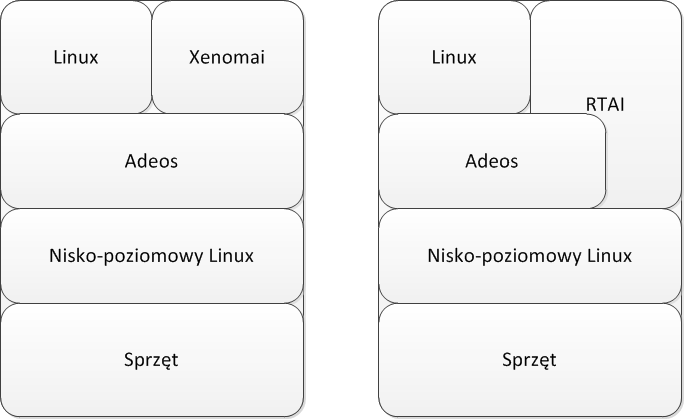
\includegraphics[width=300px]{img/XenomaiRTAI}
\caption{Architektura Xenomai i RTAI}
\label{XenomaiRTAI}
\end{center}
\end{figure}

Propagacja przerwań odbywa się za pośrednictwem kolejki. Kolejka jest łańcuchem (ang. \emph{pipeline}) systemów operacyjnych, które są kolejno budzone w reakcji na otrzymane przerwanie. W przypadku Xenomai jest on umieszczony na początku kolejki i obsługuje przerwania związane z zadaniami czasu rzeczywistego. RTAI, zgodnie ze swoją polityką maksymalnej redukcji opóźnień, samodzielnie przyjmuje przerwania, a kolejki Adeos używa jedynie do dalszej propagacji nieobsłużonych przerwań (\ref{XenomaiRTAI}). 

Warto wspomnieć również o udostępnianej w środowisku Xenomai opcji \emph{skórek RTOS} (ang. \emph{real-time operating system skins}). Pozwalają one na wybór API, z którego będą korzystać uruchamiane w Xenomai aplikacje. Do wyboru są przykładowo skórki VxWorks, co ukazuje tendencje rozwoju w stronę przenośności rozwiązania.

\subsection{Porównanie Linux 2.6, Xenomai, RTAI i VxWorks.}

Z dostępnego w publikacji \cite{pub:Comparison} zestawienia systemów wynika głównie, że w prostym scenariuszu, kiedy znana jest liczba (w tym przypadku wyłącznie jedna) i rodzaj pracujących aplikacji czasu rzeczywistego, system Linux w wersji 2.6 spisuje się zadowalająco w roli systemu o łagodnych ograniczeniach czasowych. W przypadku jądra systemu Linux 2.6 razem z liczbą i stopniem skomplikowania uruchamianych aplikacji rośnie również ilość kodu do przeanalizowania, w celu zapewnienia całkowitego determinizmu operacji, co szybko staje się niepraktyczne.

Interesujący jest dla mnie fakt, że gdy w rolę wchodzi dodatkowo komunikacja sieciowa, systemy \emph{open-source} (RTAI i Xenomai) spisują się znacznie lepiej od VxWorks. Mniejsze opóźnienia są spowodowane wykorzystaniem modułu RTnet, który przebudowuje standardowy stos IP systemu Linux pod kątem deterministycznej pracy.

%%%%%%%%%%%%%%%%%%%%%%%%%%%%

\section{Standardy 802.11 w systemach czasu rzeczywistego.}

Ze względu na swój charakter komunikacja bezprzewodowa jest nieprzewidywalna. Nie jesteśmy w stanie z góry założyć, ze sygnał nie zostanie zakłócony i informacja dotrze do celu. Pocieszający jest fakt, że na przestrzeni lat standard 802.11 podlegał wielu modyfikacjom i poprawkom (np. 802.11e, 802.11n). Część z tych aktualizacji dedykowana była możliwości zastosowania medium bezprzewodowego do komunikacji systemów czasu rzeczywistego. Koncentrują się one na potrzebie zapewnienia takiemu systemowi okien dostępu bezkolizyjnego i nadawaniu priorytetów w ruchu sieciowym. Zabiegi te pozwalają na osadzenie komunikacji systemów czasu rzeczywistego w zakłóconym paśmie transmisyjnym oraz ich koegzystencję z innymi stacjami. 

Niniejszy rozdział poświęcony jest przeglądowi dostępnych rozwinięć standardu 802.11 pod kątem użyteczności w komunikacji systemów czasu rzeczywistego.

\subsection{Problemy w 802.11 MAC - opcja DCF.}

Podstawowa wersja protokołu dostępu do medium (ang. \emph{Distributed Coordination Function}, w skrócie DCF) nie uwzględnia możliwości ustalenia priorytetów. Brak priorytetów na poziomie MAC w oczywisty sposób utrudnia realizację przewidywalnej komunikacji w systemie czasu rzeczywistego. System musiałby konkurować ze wszystkimi innymi stacjami (nawet tymi, które nie są świadome jego istnienia, a więc wprowadzają wyłącznie zakłócenia). 

Dodatkowo, stacje, które przy próbie dostępu napotkały zajęty kanał transmisji, muszą odczekać pewien losowy okres czasu (ang. \emph{Backoff}). Długość okresu oczekiwania obliczana jest jako iloczyn losowej wartości z zakresu od zera do ustalonej długości CW (ang. \emph{Contention Window}) i czasu podróży ramki w łączu (ang. \emph{Slot Time}). Oczywiste jest, że wprowadzenie losowego parametru kłóci się z ideą deterministycznej pracy.

\subsection{802.11 MAC - opcja PCF.}

Część powyżej przedstawionych problemów jest adresowana przez wprowadzenie protokołu dostępu PCF (ang. \emph{Point Coordination Function}). Opcja ta wyróżnia jedną stację (typowo jest to punkt dostępu - AP), która pełni rolę koordynatora komunikacji. Koordynator uzyskuje dostęp do łącza częściej, gdyż jego czas oczekiwania między kolejnymi ramkami jest krótszy. Po uzyskaniu dostępu do łącza koordynator wybiera stację, która może rozpocząć transmisje w oknie bezkolizyjnym. 

W tym przypadku problemem jest fakt, że nadająca stacja może wysłać ramkę arbitralnej długości. Punkt dostępowy rozsyła z okresem TBTT (ang. \emph{Target Beacon Transmission Time}) ramki typu \emph{Beacon} 
porządkujące transmisję danych. Przykładowo w 802.11e ramki \emph{Beacon} zawierają ustawienia parametrów (np. TXOP) i
informują inne stacje o zakończeniu okresu dostępu bezkolizyjnego.
Protokół dostępu PCF nie posiada ograniczeń, które mogłyby powstrzymać stację przed pogwałceniem okresu TBTT. Jest
możliwe, że stacja, która została wybrana przez AP w okresie dostępu bezkolizyjnego rozpocznie przesyłanie zbyt dużych ramek,
których czas przesyłania przekroczy czas okresu TBTT. Przekroczenie czasu TBTT powoduje, że AP opóźni propagację ramek
\emph{Beacon}. Brak możliwości deterministycznego określenia długości trwania okresu dostępu bezkolizyjnego, czy też samego
czasu transmisji pojedynczej stacji w tym okresie powoduje, że obsługa komunikacji systemów czasu rzeczywistego za pomocą
protokołu PCF jest utrudniona.

\subsection{Wsparcie dla QoS w standardzie 802.11e.}

Standard 802.11e wprowadził nowy protokół dostępu EDCA (ang. \emph{Enhanced Distributed Channel Access}). Protokół ten udostępnia 4 klasy priorytetów dla ruchu. System priorytetów zbudowany jest na bazie parametrów odziedziczonych po protokole DCF. 

Każda klasa dostępu posiada własny odstęp międzyramkowy AIFS (ang. \emph{Arbitration Interframe Space}).

Czas \emph{Backoff} nadal wyliczany jest w sposób losowy, ale w tym przypadku jest to wartość z przedziału od zera do górnej granicy, która na wstępie wynosi CWmin. W sytuacji dużej zajętości medium, kiedy stacja natrafia na zajęty kanał to wartość maksymalna jest zwiększana, ale nie wyniesie więcej niż CWmax (CWmin i CWmax są parametrami ustalanymi indywidualnie dla każdej klasy dostępu).

Może dojść do sytuacji, kiedy natężenie ruchu w sieci komunikacyjnej jest na tyle duże, że priorytety nie wystarczają dla zapewnienia odpowiedniej jakości połączenia dla systemu czasu rzeczywistego. W takiej sytuacji możliwe jest użycie parametru TXOP (ang. \emph{Transmission Oportunity}). 

Parametr TXOP pozwala stacji na transmisję serii ramek (ang. \emph{burst}). Po uzyskaniu dostępu do łącza
węzeł może przesyłać kolejne ramki z odstępem SIFS (ang. \emph{short interframe space}) między porcją danych, a
ramką potwierdzenia ACK. TXOP zapewnia bezkolizyjny dostęp do medium jednocześnie ograniczając maksymalny czas 
okresu dostępu bezkolizyjnego dla danej stacji. Jeśli przesyłanie ramki trwałoby dłużej niż czas TXOP to ramka
ta zostanie podzielona, aby zachować jakość usług.

Podsumowując, istnieją 4 parametry podlegające niezależnej regulacji w ramach każdej z klas dostępu:

\begin{itemize}
\item CWmin - minimalna długość losowego składnika czasu \emph{Backoff}.
\item CWmax - maksymalna długość losowego składnika czasu \emph{Backoff}.
\item AIFSN - Składnik odstępu międzyramkowego. 
\item Max TXOP - Maksymalny czas dostępu bezkolizyjnego po uzyskaniu medium.
\end{itemize}

Ostateczna długość \eqref{eq:AIFS} odstępu międzyramkowego AIFS (ang. \emph{Arbitration Inter-frame Spacing}) wyliczana jest poprzez sumowanie czasu SIFS (ang. \emph{Shot Inter-frame Spacing}), który jest wartością stałą, z iloczynem AIFSN (Składnik odstępu międzyramkowego dla danej klasy dostępu) i czasu podróży danych w łączu (ang. \emph{Slot Time}). Czas SIFS jest najkrótszym z dostępnych w specyfikacji odstępów międzyramkowych.    

\begin{figure}
\caption{Wzór na odstęp międzyramkowy.}
\begin{equation} 
\label{eq:AIFS}
AIFS = SIFS + AIFSN * Slot Time 
\end{equation}
\end{figure}

Warto zauważyć, że zmniejszanie czasów oczekiwania rywalizującej stacji umożliwia jej częstszy
dostęp do medium, lecz powoduje również wzrost kolizji na łączu. Wynika z tego, że w celu stworzenia dogodnego środowiska dla pracy systemu czasu rzeczywistego należy ograniczyć liczbę stacji obsługiwaną przez dany punkt dostępowy. W sytuacji osiągnięcia maksimum \emph{AP} nie musi wykonywać już procesu asocjacji. Parametr ten powinien być łatwo dostępny w większości interfejsów obsługi punktów dostępowych (przykładowo w pliku konfiguracyjnym demona \emph{hostapd} służy do tego wartość \emph{max\_num\_sta}).

\subsection{Zastosowanie 802.11e w przykładowym środowisku.}

Standard 802.11e udostępnia następujące klasy dostępu:

\begin{itemize}
\item AC\_VO - klasa dostępu głosowego (najwyższy priorytet)
\item AC\_VI - klasa dostępu wideo
\item AC\_BE - klasa ruchu uprzywilejowanego 
\item AC\_BK - ruch w tle (najniższy priorytet)
\end{itemize}

W tym przypadku system czasu rzeczywistego mógłby korzystać z klasy AC\_VO (\cite{pub:802.11e}). Inne stacje świadome istnienia systemu mogą komunikować się w klasie AC\_BK. Jeśli chodzi o stacje nieświadome istnienia systemu to można dla nich przeznaczyć klasę AC\_BE.

\subsection{Rozwiązania na poziomie oprogramowania Linux.}

Mechanizm QoS (ang. \emph{Quality Of Service}) jest realizowany w jądrze 2.6 w postaci struktury komponentów, z których każdy realizuje pewien podzbiór funkcjonalności związanych z sterowaniem ruchem sieciowym (\cite{pub:QoS}). Główne składniki modułu QoS w systemie Linux to:

\begin{itemize}
\item qdisc - odpowiada za politykę kolejkowania ramek na urządzeniu.
\item class - umożliwia podział pakietów na klasy priorytetów w ramach qdisc.
\item filter - jest elementem odpowiadającym za podział na klasy lub np. upuszczanie ramek.
\end{itemize}

Wstępnie dostępne są dwa elementy qdisc - ingress i root (egress). Główna funkcjonalności skupia się w qdisc'u root, gdyż odpowiada on za kolejkowanie ramek wychodzących ( qdisc ingress umożliwia jedynie np. proste upuszczanie ramek ).

Istnieją dwa typy komponentów qdisc - korzystający z klas (ang. \emph{classfull qdisc}) i nie korzystający z klas (ang. \emph{classless qdisc}). 

Qdisc nie wykorzystujący klas pozwala na realizację prostej polityki kolejkowania typu FIFO (ang. \emph{First-in-first-out}). Standardowo, system Linux do kolejkowania swoich ramek wykorzystuje qdisc typu \emph{pfifo\_fast}, która składa się z trzech kolejek FIFO opróżnianych wedle swojego priorytetu. \emph{Classless qdisc} pozwala na realizację prostej polityki ograniczania częstotliwości ramek. TBF (ang. \emph{Token Bucket Filter}) bazuje na buforze wypełnianym małymi porcjami danych (żetonami), które są konsumowane przez wysyłane ramki.

Qdisc korzystający z klas pozwala na implementację bardzo skomplikowanych struktur drzewiastych (ang. \emph{Hierachical Token Bucket}). Każda klasa może zawierać inne klasy, przy czym w liściach drzewa następuje kształtowanie ruchu (znajdują się tam elementy qdisc). Klasy służą jedynie do odpowiedniego podziału dostępnych żetonów. Zaimplementowano również mechanizm pożyczania. Jeśli klasa dziecko wyczerpała dostępne żetony, to pożycza je od klasy rodzica.

\subsection{Stos IP RTnet.}

RTnet jest nowym stosem IP przeznaczonym dla systemów Xenomai i RTAI. Zastępuje on standardowy stos systemu Linux i wprowadza zmiany istotne z punktu widzenia komunikacji systemów czasu rzeczywistego.

Bufor pakietu \emph{sk\_buff} został zastąpiony przez strukturę \emph{rtskb}, która ma następujące własności:

\begin{itemize}
\item Stały rozmiar (zawsze maksymalny)
\item Pula buforów jest alokowana na początku działania systemu dla każdej warstwy stosu
\item Bufory są przekazywane między warstwami na zasadzie wymiany
\end{itemize}

Wymiana buforów \emph{rtskb} jest konieczna ze względu na potrzebę utrzymania zapasu wskaźników na alokowaną pamięć dostępną w puli danej warstwy stosu.

Inną ważną cechą RTnet jest fakt, że implementacja UDP/IP odbywa się poprzez statyczne przypisanie adresów (nie korzysta z protokołu ARP). Dla pakietów IP przesyłanych we fragmentach potrzebne bufory \emph{rtskb} pobierane są z puli globalnej.



\chapter{Pomiar czasu przełączania kanału radiowego.}
%

Ciężko uniknąć sytuacji, w której systemy wykorzystujące do komunikacji standard \emph{802.11} napotykają potrzebę zmiany częstotliwości (przełączenia kanału) pracy swoich interfejsów kart radiowych NIC (ang. \emph{Network Interface Card}). Główną przyczyną podziału pasma jest wielodostęp, a więc unikanie wzajemnego zakłócania się urządzeń. Należy wziąć pod uwagę, że medium transmisyjne w środowisku przemysłowym jest zwykle wyjątkowo zaszumione w paśmie \emph{2.4 GHz}. Dla uzmysłowienia stopnia zakłóceń wystarczy wymienić część urządzeń pracujących w paśmie \emph{ISM} (ang. \emph{Industrial, scientific and medical}) takich jak:
\begin{itemize}
\item[--] elektroniczne nianie,
\item[--] urządzenia Bluetooth,
\item[--] kuchenki mikrofalowe,
\item[--] alarmy samochodowe
\end{itemize}
Łatwo zauważyć jak bardzo zróżnicowane urządzenia mogą doprowadzić do problemów w bezprzewodowej komunikacji systemów czasu rzeczywistego.

Warto wspomnieć, że istnieje już specyfikacja standardu pracującego w paśmie \emph{5 GHz} (\cite{std:IEEE80211n}), lecz nie jest on jeszcze powszechnie wspierany. Biorąc za przykład rozwiązania \emph{open-source} można zauważyć, że standard \emph{802.11n} jest obsługiwany przez nowe sterowniki (\emph{ath9k} dla urządzeń firmy \emph{Atheros}). Problemem jest natomiast fakt, że tego typu sterowniki dostępne są jedynie w najnowszych dystrybucjach systemów operacyjnych przeznaczonych dla urządzeń wbudowanych (przykładowo \emph{OpenWrt Backfire 10.03}), które nie zawsze od początku wspierają zadowalającą gamę urządzeń. Dla przykładu nadal istnieją problemy z dostępnością tego typu sterowników dla popularnej płytki \emph{MagicBox}.

Biorąc pod uwagę fakt zaszumienia medium transmisyjnego wnioskuję, że możliwość zmiany częstotliwości pracy interfejsu \emph{NIC} w poszukiwaniu dogodnego kanału komunikacji jest jedną z jego kluczowych i wymagających uwagi cech. W ostatnich latach powstało wiele publikacji dotyczących możliwości adaptacji struktury sieci bezprzewodowych do panującej jakości medium komunikacyjnego (\cite{pub:DCS}). Prace te koncentrują się głównie na algorytmach dynamicznej modyfikacji częstotliwości pracy interfejsów w sieciach kratowych \emph{WMN} (ang. \emph{Wireless Mesh Network}). Oczywiście u podstaw zastosowanych rozwiązań leży zjawisko przełączania kanału radiowego.

Powyższe czynniki sugerują, że całkowite wyeliminowanie potrzeby przełączania kanału (zmiany częstotliwości pracy) interfejsów radiowych nie jest aktualnie osiągalne. Co więcej, udostępnianie nowych pasm częstotliwości, w sytuacji ciągle rosnącego zapotrzebowania, jest jedynie tymczasowym rozwiązaniem.  


% Rozwiązanie z 2-3 interfejsami radiowymi ???
\section{Przełączanie kanału radiowego.}
Opóźnienie związane ze zmianą częstotliwości pracy jest ważnym parametrem, gdyż w tym czasie stacja zaprzestaje reakcji na kierowane do niej dane. Ramki skierowane do stacji są tracone co w oczywisty sposób może wpłynąć na ograniczenia czasowe, w których działają komunikujące się systemy. 
Typowe scenariusze, w których może zajść potrzeba zmiany częstotliwości pracy interfejsu NIC to:
\begin{itemize}
\item[--] Stacja kliencka w trybie \emph{Managed} dokonuje \emph{Roamingu} między dwoma punktami dostępowymi AP (ang. \emph{Access Point}) 
\item[--] Stacja kliencka w trybie \emph{Managed} skanuje medium w poszukiwaniu punktów dostępowych AP (ang. \emph{Access Point})
\item[--] Stacja kliencka w trybie \emph{Ad-hoc} skanuje medium po aktywacji interfejsu lub samym przełączeniu kanału 
\end{itemize}
Identyfikacja powyższych sytuacji to pierwszy krok ku specyfikacji konkretnych scenariuszy pomiarowych. 

Najczęstszą przyczyną przełączania kanału jest procedura skanowania medium komunikacyjnego. Podczas skanowania stacja wysyła ramki typu \emph{Probe Request} na każdej z dostępnych w specyfikacji (\cite{std:IEEE80211}) częstotliwości pracy i oczekuje na ramki \emph{Probe Response} od punktów dostępowych, lub stacji w trybie \emph{Ad-hoc} (w zależności od typu interfejsu NIC, czyli rodzaju docelowej sieci).

Przełączanie kanału następuje również, kiedy stacja kliencka oddala się zbyt daleko od punktu dostępowego i musi rozpocząć poszukiwanie nowego w swoim zasięgu. Jest to sytuacja zwana roamingiem i wymaga uwagi podczas rozważania systemów, w których skład wchodzą mobilne stacje, czy agenci. Obszar działania systemu może być na tyle różnorodny pod względem zakłóceń, że konieczne będzie przełączanie kanału między kolejnymi punktami dostępowymi pracującymi na różnych częstotliwościach.

\section{Metodyka pomiaru.}
Z punktu widzenia zjawiska komunikacji w standardzie 802.11 za kluczową uznałem możliwość prowadzenia pomiarów z minimalną ingerencją w strukturę i działanie stacji. Osiągnięcie tego celu wymaga uruchomienia dodatkowej maszyny, która prowadzi nasłuch w medium komunikacyjnym. Jedną z zalet tego typu rozwiązania jest fakt, że programistyczne środowisko pomiarowe przygotowuję tylko na jednej stacji. Jest to niezwykle ważne w przypadku, gdy w danym scenariuszu pomiarowym biorą udział systemy wbudowane (np. pełniące funkcję routerów) z ograniczonymi możliwościami instalacji rozbudowanych aplikacji i bibliotek programistycznych. 

Warto zauważyć, że stacje mogą pracować na różnych częstotliwościach i zmieniać je w trakcie trwania obserwacji. Stacja pomiarowa, będąca w posiadaniu informacji na temat aktualnie badanego zjawiska, musi mieć możliwość zmiany kanału pracy swojego interfejsu nasłuchującego w sposób, który nie spowoduje utraty informacji z łącza. Jednym z rozwiązań tego problemu jest zastosowanie wielu interfejsów radiowych, które podczas inicjalizacji procedury pomiarowej wprowadzane są na częstotliwości pracy przeznaczone do obserwacji konkretnych uczestników. 

Opis stosowanych metodyk pomiarowych rozpocznę od definicji podstawowych pojęć opisujących środowisko i uczestników scenariuszy. Najważniejsze pojęcia to:
\begin{itemize}
\item[--] {\bf Stacja pomiarowa}: Komputer działający pod kontrolą interakcyjnego systemu operacyjnego, na którym uruchomiona jest aplikacja nasłuchująca ruch sieciowy (ang. \emph{sniffer}).
\item[--] {\bf Stacja kliencka}: Komputer pełniący rolę klienta w sieci o strukturze wykorzystującej punkty dostępowe (ang. \emph{Infrastructure mode}). Może być to zarówno komputer pod kontrolą systemu interakcyjnego, lub wbudowanego.
\item[--] {\bf Punkt dostępowy}: Komputer pełniący w trybie infrastruktury (ang. \emph{Infrastructure mode}) rolę stacji AP (ang. \emph{Access Point}). Może być to zarówno komputer pod kontrolą systemu interakcyjnego, lub wbudowanego.
\item[--] {\bf Rozwiązanie asocjacji}: Zdarzenie wysłania ramki rozwiązującej asocjację między stacją kliencką, a punktem dostępowym (ang. \emph{Disassociation frame}).
\item[--] {\bf Skanowanie}: Wysyłanie przez stację ramek typu \emph{Probe Request} na wszystkich dostępnych w specyfikacji (\cite{std:IEEE80211}) częstotliwościach pracy.
\item[--] {\bf Scenariusz pomiaru}: Jeden ze scenariuszy możliwych do zaistnienia podczas komunikacji stacji w standardzie 802.11, w którego czasie następuje przełączenie kanału interfejsu NIC.
\item[--] {\bf Zdarzenie}: Przechwycenie ramki standardu 802.11 biorącej udział w scenariuszu pomiarowym. 
\end{itemize}

\section{Scenariusz pomiaru: Roaming 802.11.}
Roaming 802.11 to zjawisko zachodzące w sieciach, w trybie infrastruktury (ang. \emph{Infrastructure mode}). Podstawowym celem jest umożliwienie stacji klienckiej odłączenia się od punktu dostępowego i podjęcia próby odnalezienia i podłączenia się do stacji o mocniejszym sygnale. W warunkach rzeczywistych sytuacja taka najczęściej jest wynikiem ruchu mobilnej stacji klienckiej (np. przemieszczającego się pracownika biura, lub agenta w systemie przemysłowym), która dociera do granicy zasięgu dotychczas używanego punktu dostępowego. Aby zachować połączenie z systemem, lub usługami (np. dostęp do internetu) maszyna musi odnaleźć inną stację pracującą w trybie AP o mocniejszym sygnale. Na procedurę roamingu 802.11 składają się następujące kroki:
\begin{itemize}
\item[--] Stacja kliencka wykrywa, że poziom sygnału RF (ang. \emph{Radio Frequency})
punktu dostępowego \#1 jest poniżej progu roamingu.
\item[--] Stacja kliencka rozpoczyna nadawanie ramek rozwiązujących asocjację do punktu dostępowego \#1 do momentu potwierdzenia odebrania.
\item[--] Punkt dostępowy \#1 otrzymuje ramkę rozwiązującą asocjację \emph{Disassociation frame} i usuwa stację kliencką z tablicy asocjacji.
\item[--] Stacja kliencka rozpoczyna skanowanie medium komunikacyjnego i oczekuje ramek \emph{Probe Response}.
\item[--] Punkt dostępowy \#2 wysyła do stacji klienckiej ramkę typu \emph{Probe Response}.
\item[--] Stacja kliencka rozpoczyna wysyłanie do punktu dostępowego \#2 ramek typu \emph{Association request}.
\item[--] Punkt dostępowy \#2 dokonuje asocjacji stacji klienckiej i potwierdza to zdarzenie wysyłając ramkę typu \emph{Association response}.
\end{itemize}

Łatwo zauważyć, że zjawisko roamingu jest kluczowe w przypadku systemu czasu rzeczywistego zarządzającego stacjami mobilnymi na rozległym obszarze (\ref{MobileAgentSystem}). System może wykorzystywać wiele punktów dostępowych, które obsługuje poprzez sieć przewodową (ang. \emph{Ethernet}). Każda zarządzana stacja w trybie AP przystosowana jest do działania w panujących na swoim obszarze warunkach zaszumienia łącza. Roaming 802.11 byłby w tym wypadku główną przyczyną przełączania kanału radiowego interfejsu NIC w mobilnych stacjach klienckich. 

\begin{figure}[htb]
\begin{center}
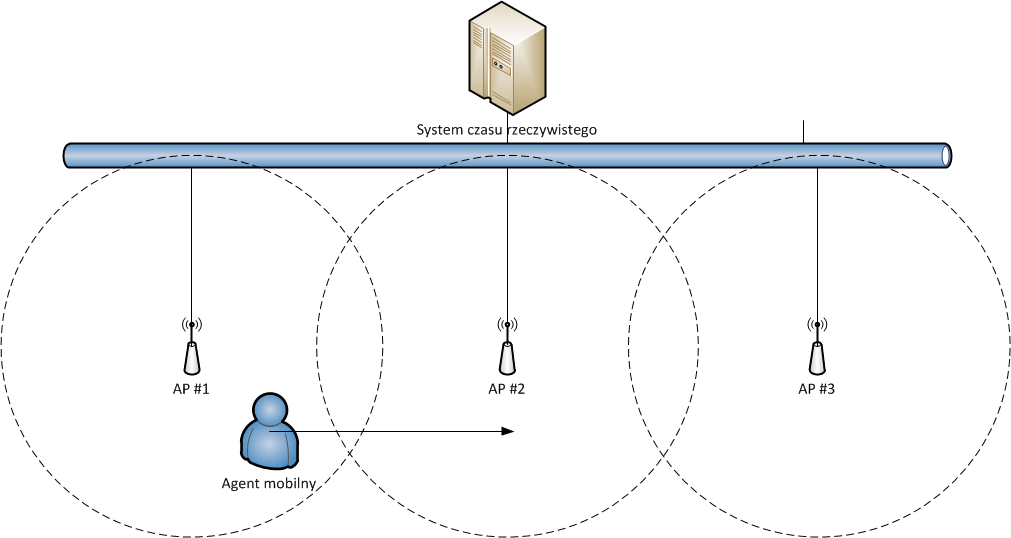
\includegraphics[width=250px]{img/System_czasu_rzeczywistego}
\caption{System z mobilnym agentem}
\label{MobileAgentSystem}
\end{center}
\end{figure}

Oczywiście roaming nie implikuje ruchu żadnej z maszyn, co ułatwia przeprowadzenie pomiaru. Wystarczy doprowadzić do sytuacji, w której moc sygnału punktu dostępowego spadnie poniżej progu (ang. \emph{roaming threshold}), który powoduje decyzję o rozwiązaniu asocjacji stacji klienckiej. 

\begin{figure}[htb]
\begin{center}
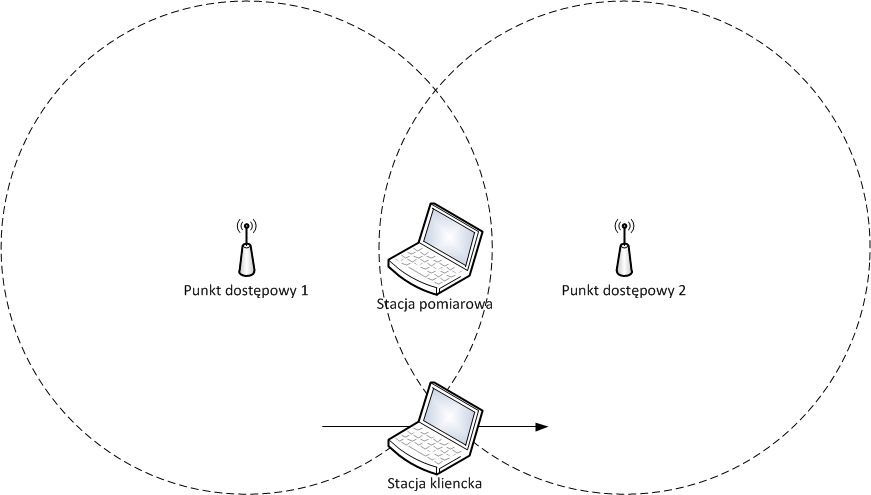
\includegraphics[width=250px]{img/Roaming}
\caption{Roaming 802.11: Środowisko pomiarowe.}
\label{RoamingEnviroment}
\end{center}
\end{figure}

\subsection{Środowisko pomiarowe.}
\label{sec:MeasurementEnviroment}

W skład środowiska pomiarowego (\ref{RoamingEnviroment}) wchodzą dwa punkty dostępowe, stacja kliencka oraz stacja pomiarowa. Punkty dostępowe pracują na różnych częstotliwościach. Do wyboru, zgodnie ze standardem 802.11g (\cite{std:IEEE80211}), są kanały numer 1, 5, 9, lub 13. Są to nienachodzące na siebie zakresy częstotliwości. W celu ułatwienia roamingu stacja kliencka umieszczona jest na granicy zasięgu punktów dostępowych. Stacja pomiarowa musi znajdować się w zasięgu stacji klienckiej, oraz obydwu punktów dostępowych (musi być w stanie rejestrować ruch sieciowy). 
Należy zwrócić uwagę na zapewnienie odpowiedniej jakości medium transmisyjnego. Wysoki poziom zakłóceń na kanałach wykorzystywanych w eksperymencie wprowadzi zakłamania, jeśli interesuje nas wyłącznie czas trwania samej procedury roamingu. 

\subsection{Mierzona wartość: Czas roamingu.}
Czas roamingu 802.11 rozumiem jako czas (\ref{RoamingTime}) mierzony od momentu decyzji stacji klienckiej o zaprzestaniu normalnej wymiany danych z punktem dostępowym do momentu powiązania z nową stacją w trybie AP o mocniejszym sygnale. Zdarzeniem inicjującym pomiar jest wysłanie przez stację kliencką pierwszej ramki rozwiązującej asocjację (ang. \emph{Disassociation frame}). Pomiar zostaje zakończony w momencie wysłania przez nowy punkt dostępowy ramki potwierdzającej asocjację nowej stacji (ang. \emph{Association Response frame}).

Podstawowa procedura pomiarowa składa się z następujących kroków:
\begin{itemize}
\item[--] Stacja kliencka przeprowadza asocjację z punktem dostępowym 1.
\item[--] Stacja kliencka przemieszcza się poza zasięg punktu dostępowego 1 i wykonuje procedurę roamingu do punktu dostępowego 2.
\item[--] Stacja pomiarowa wykrywa próbę rozwiązania asocjacji i rozpoczyna pomiar czasu.
\item[--] Punkt dostępowy 2 dokonuje asocjacji stacji klienckiej.
\item[--] Stacja pomiarowa rejestruje potwierdzenie asocjacji stacji klienckiej i zatrzymuje pomiar czasu.
\end{itemize}

\begin{figure}[htb]
\begin{center}
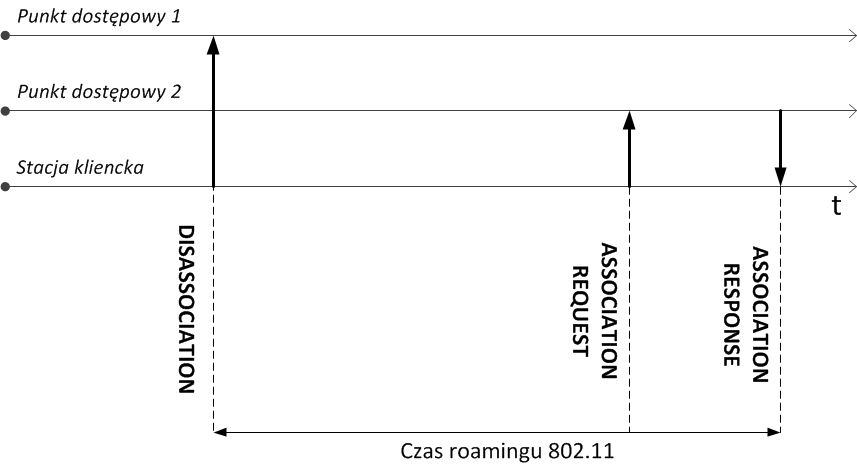
\includegraphics[width=250px]{img/RoamingTime}
\caption{Roaming 802.11: Czas roamingu.}
\label{RoamingTime}
\end{center}
\end{figure}

\subsection{Wymagania co do aplikacji \emph{hop-sniffer}.}
\label{sec:ApplicationRequirements}

Do przeprowadzenia powyżej zdefiniowanej procedury pomiaru opóźnienia roamingu stacji klienckiej niezbędne jest wytworzenie oprogramowania pomocniczego. Aplikacja ta działa w środowisku stacji pomiarowej i służy do przechwytywania i reagowania na zdarzenia scenariusza. Powinna ona spełniać wszelkie wymagania funkcjonalne i niefunkcjonalne stawiane przez procedurę pomiarową. W wyniku analizy zidentyfikowałem następujące wymagania: 
\begin{enumerate}
\item Architektura aplikacji nie jest rozproszona na wielu maszynach.
\item Aplikacja działa na komputerze przenośnym.
\item Aplikacja umożliwia przechwytywanie ramek zarządzających komunikacją standardu 802.11 (ang. \emph{Management}). 
\item Przechwytywane ramki muszą pochodzić z dowolnej sieci i adresów MAC (\emph{Media Access Control}).
\item Przechwytywanie musi odbywać się z minimalną ingerencją w badaną architekturę komunikacyjną.
\item Aplikacja przetwarza i buduje swoją logikę działania na podstawie zawartości nagłówków i pól danych pakietów. 
\item Dokładność pomiaru czasu musi być większa od interwałów występowania zdarzeń standardu 802.11.
\item Pomiar czasu musi być wykonany w zdefiniowanym momencie na określonym poziomie modelu stosu \emph{TCP/IP}.
\end{enumerate}

Scentralizowana architektura aplikacji oznacza działanie jej składników wyłącznie na stacji pomiarowej. Oznacza to, że wszelkie biblioteki i narzędzia programistyczną muszą być dostępne tylko na jednej maszynie. Ułatwia to przeprowadzenie pomiaru z udziałem dowolnych stacji (np. systemów wbudowanych uniemożliwiających instalację własnego oprogramowania). Eliminacji ulega również dodatkowy i ciężki do oszacowania narzut związany z komunikacją elementów samego systemu pomiarowego.

Działanie na komputerze przenośnym jest podyktowane łatwą organizacją określonego w specyfikacji środowiska. Stacja pomiarowa musi znajdować się w zasięgu wszystkich uczestników obserwowanego scenariusza, więc możliwa powinna być łatwa manipulacja jej położeniem.

Obserwacja opóźnień dowolnego zjawiska w standardzie 802.11 wymaga dostępu do elementarnych zdarzeń sterujących jego przebiegiem. Pochodną tego wymagania jest potrzeba nasłuchiwania w medium transmisyjnym w celu przechwytywania nie tyle ramek danych, co ramek porządkujących cały proces komunikacji (ang. \emph{Management frames}). Za ich pomocą stacje informują innych uczestników protokołu komunikacyjnego o rozpoczęciu, przebiegu i zakończeniu roamingu i innych opisanych w standardzie zjawisk. 

Niezwykle ważna jest konieczność obejścia dwóch niskopoziomowych filtrów pakietów, które stoją na przeszkodzie obserwacji wszystkich zdarzeń. Filtry te służą zwiększeniu wydajności komunikacji poprzez wczesne odrzucenie pakietów, które z pewnością nie interesują danej stacji. Pierwszym z nich jest filtr adresów \emph{MAC}, który odrzuca wszystkie ramki nie kierowane do danego interfejsu. Kolejnym jest filtr identyfikatorów \emph{SSID} (ang. \emph{Service Set Indetifier}), który upuszcza pakiety nie pochodzące z infrastruktury, której stacja nie jest członkiem. Stacja pomiarowa nie powinna być w asocjacji z żadnym punktem dostępowym, ale być w stanie przechwycić komunikaty pochodzące z dowolnego \emph{AP} (ang. \emph{Access Point}). 

Wymaganie co do minimalnej ingerencji w środowisko pomiarowe wynika z charakteru medium transmisyjnego. Interfejs stacji pomiarowej nie powinien pracować w żadnym trybie, który implikuje okresowe rozsyłanie ramek (przykładowo ramki typu \emph{Beacon} dla trybu \emph{AP}). Stacja nie powinna również podejmować prób asocjacji z punktami dostępowymi biorącymi udział w eksperymencie, aby nie wprowadzać dodatkowych opóźnień w pracy ich oprogramowania. Dopuszczalne jest rozesłanie ramek \emph{Probe Request} w fazie inicjalizacji środowiska w celu rozpoznania warunków panujących w medium transmisyjnym (moc nadawania, częstotliwości pracy poszczególnych interfejsów \emph{NIC}). 

Aplikacja działa na zasadzie reakcji na wartości odczytane z pól nagłówków i danych przechwyconych ramek. Powinna różnicować swoje zachowanie w zależności od tych informacji w celu realizacji zadanego scenariusza pomiarowego.

Dokładność pomiaru czasu przez aplikację \emph{hop-sniffer} musi być większa od podstawowej jednostki czasu używanej do określania interwałów czasu w standardzie 802.11. Jednostką tą jest TU (ang. \emph{Time Unit}) o długości 1024 mikrosekund. Specyfikacja taka wynika z potrzeby uniknięcia stosowania milisekund trudniejszych do odmierzenia w systemach mikroprocesorowych. Przyjmuję, że dokładność rzędu mikrosekund jest wystarczająca. Rząd milisekund może być nieodpowiedni ze względu na problem ze śledzeniem jednostki TU. Milisekunda nie mieści się w dowolnej mierze określonej w TU całkowitą liczbę razy. 

Aplikacja mierzy czas między zdarzeniami zdefiniowanymi jako fakt odebrania ramki określonego typu. Moment wystartowania licznika, bądź zebrania stempla czasowego na drodze ramki przez stos \emph{TCP/IP} powinien być jasno określony. Jeśli stacja pomiarowa działa pod kontrolą systemu operacyjnego pracującego w sposób niedeterministyczny to można spodziewać się trudnych w oszacowaniu opóźnień podczas uruchamiania licznika w warstwie aplikacyjnej.  





\chapter{Narzędzie pomiarowe: \emph{hop-sniffer}.}
%
 
Niniejszy rozdział poświęcony jest opisowi aplikacji powstałej na podstawie wymagań sformułowanych w opisie pomiaru \ref{sec:ApplicationRequirements}. Analiza wymagań podyktowała stworzenie programu, który umożliwiałby pogląd ramek zarządzających komunikacją w standardzie 802.11 (ang. \emph{Management frames}) oraz analizę zależności czasowych między nimi. 

Wymagane okazało się stworzenie aplikacji nasłuchującej (ang. \emph{sniffer}) przystosowanej do obserwacji typowych scenariuszy zachodzących w komunikacji w medium bezprzewodowym. Przystosowanie to rozumiem jako możliwość konfiguracji programu pod kątem wybranego zjawiska i środowiska pomiarowego. 

Część tego rozdziału poświęcona jest opisowi dwóch bibliotek programistycznych pod kątem ich zastosowania do przechwytywania pakietów. \emph{Libnl} jest biblioteką bardziej ogólną niż \emph{libpcap}. Implementacja nasłuchiwania z jej udziałem napotkała problemy, które wymusiły przejście programu na bibliotekę \emph{libpcap}. \emph{Libnl} pozwala jednak na programistyczne nadawanie ramek typu MGMT (ang. \emph{Management}) co otwiera możliwość testowania rozwiązania \emph{hop-sniffer}.

\section{Środowisko pracy programu.}
\label{sec:ProgramEnviroment}

Program hop-sniffer został przygotowany dla systemu operacyjnego Linux w wersji jądra 2.6. W wyborze systemu operacyjnego kierowałem się głównie metodą implementacji sterowników urządzeń bezprzewodowych i obsługującej je warstwy pośredniej jądra. 

System Linux był wyborem oczywistym ze względu na możliwość konfiguracji interfejsów NIC w sposób umożliwiający przetwarzanie ramek typu MGMT (ang. \emph{management}) standardu 802.11 za pomocą aplikacji w przestrzeni użytkownika.

Kolejną zaletą wybranego systemu jest możliwość konfiguracji najbardziej odpowiedniej dystrybucji i kompilacji powstałego rozwiązania jedynie z użyciem opcji dedykowanych dla aplikacji pomiarowej. W tym wypadku najbardziej pożądane jest minimalistyczne środowisko, które w możliwie najmniejszym stopniu wpływało będzie na prezentowane przez program wyniki pomiarów. Jako środowisko zalecane wybrałem system Arch Linux \cite{www:ArchLinux}.

Biorąc pod uwagę program komunikujący się z kartą radiową w systemie Linux należy zwrócić szczególną uwagę na kwestię sterowników. Od sterowników urządzeń bezprzewodowych zależy jakie polecenia i tryby pracy interfejsów będą dostępne do konfiguracji w przestrzeni użytkownika. Ze względu na aktualne dążenie programistów jądra do unifikacji interfejsu obsługi urządzeń standardu 802.11 powstała warstwa pośrednia \emph{mac80211}. Postanowiłem oprzeć aplikację hop-sniffer o sterowniki działające w tej warstwie ze względu na wspólny, oparty na gniazdach interfejs komunikacyjny \emph{nl80211}. Kluczowym wymaganiem stawianym sterownikowi jest implementacja polecenia umożliwiającego utworzenie wirtualnego interfejsu karty radiowej pracującego w trybie \emph{monitor}.

Wprowadzenie karty radiowej w tryb \emph{promiscuous} powoduje jedynie wyłączenie filtracji adresów MAC. Program hop-sniffer musi mieć możliwość odbierania ramek standardu 802.11 bez potrzeby asocjacji z SSID (ang. \emph{Service Set Identifier}) żadnej sieci. Wyłączenie filtracji SSID możliwe jest jedynie w trybie \emph{monitor}.

Skoncentrowałem się na współpracy ze sterownikiem \emph{ath9k}. Jest to całkowicie otwarty sterownik do urządzeń standardu 802.11bgn firmy \emph{Atheros}. Za wykorzystaniem sterownika przemawia dostępność wspieranych przez niego urządzeń, implementacja szerokiej gamy poleceń interfejsu \emph{nl80211} oraz możliwość pracy w trybie \emph{monitor}.

\section{Biblioteki programistyczne.}

Implementacja aplikacji pomiarowej wymagała zastosowania API (ang. \emph{Application interface}) umożliwiającego przechwytywanie ramek zarządzających komunikacją 802.11 w przestrzeni użytkownika. Podczas procesu tworzenia programu hop-sniffer rozpatrzyłem zastosowanie dwóch bibliotek: \emph{libnl} i \emph{libpcap}. Wykorzystałem materiały ze stron projektów \emph{Linux Wireless} oraz \emph{Libpcap/Tcpdump}. Strony te zawierają dokumentację bibliotek \emph{libnl} \cite{www:LibnlDoc} i \emph{libpcap} \cite{www:LibPcapDoc} oraz kody źródłowe przykładowych programów \emph{iw} \cite{www:IWSrc} i \emph{tcpdump} \cite{www:TcpDumpSrc}. 

\subsection{Nasłuchiwanie za pomocą interfejsu \emph{nl80211}.}

\emph{Libnl} jest to API (ang. \emph{Application interface}) służące do komunikacji między przestrzenią użytkownika i warstwą \emph{mac80211} jądra systemu operacyjnego. Interfejs \emph{nl80211} tej warstwy oparty jest o system gniazd \emph{Generic Netlink} (w odróżnieniu od stosowanych dawniej wywołań systemowych \emph{IOCTL}).  

Warstwa pośrednia definiuje rodzinę gniazd (ang. \emph{Generic netlink family}) oraz rejestruje w jej obrębie zestaw poleceń w postaci akceptowanych rodzajów wiadomości. Sterowniki urządzeń 802.11 implementują powyższy interfejs poprzez inicjalizację odpowiadających poleceniom wskaźników na funkcje własnymi operacjami. Każda wiadomość akceptowana przez daną rodzinę posiada własną nazwę oraz wskaźnik na strukturę określającą ilość i typy atrybutów (ang. \emph{Generic netlink attribute policy}), która pełni funkcję kontroli poprawności. Struktura ta zwana \emph{nla\_policy} stanowi wytyczne co do sposobu konstrukcji skierowanego do jądra polecenia oraz ekstrakcji danych z odebranej wiadomości.

W wyniku analizy dokumentacji uznałem, że możliwa będzie implementacja programu nasłuchującego z wykorzystaniem następujących mechanizmów udostępnianych przez interfejs \emph{nl80211}:

\begin{itemize}
\item[--] Grupowych adresów (ang. \emph{Multicast groups}) odbiorców wiadomości.
\item[--] Komendy \emph{NL80211\_CMD\_REGISTER\_FRAME}.
\item[--] Własnych funkcji obsługi zdarzeń (ang. \emph{Custom callback}).
\item[--] Komendy \emph{NL80211\_CMD\_FRAME}.
\end{itemize}

Adresy grupowe są wykorzystywane przez jądro do rozgłaszania zdarzeń warstwy \emph{mac80211} do zainteresowanych procesów (posiadających gniazdo z członkostwem w danej grupie rozgłaszania). W celu otrzymywania wszystkich zdarzeń należy zarejestrować gniazdo \ref{code:MulticastExample} we wszystkich czterech grupach: \emph{Configuration, Scan, Regulatory i MLME}. Podczas rejestracji \ref{code:MulticastExample} funkcja \emph{nl\_get\_multicast\_id(3)} przyjmuje uchwyt gniazda komunikacyjnego, nazwę rodziny, do której odnosi się zapytanie i nazwę grupy, której identyfikator chcę uzyskać. W wyniku wywołania otrzymuję liczbę całkowitą, którą mogę wykorzystać w celu rejestracji danego gniazda w grupie rozgłaszania przy pomocy funkcji \emph{nl\_socket\_add\_membership(2)}.

\lstset{caption={Przykład rejestracji gniazda w grupie \emph{Configuration}.}, label={code:MulticastExample}}
\begin{lstlisting}[frame=tb]
/* Get configuration multicast group ID */
multicast_id = nl_get_multicast_id(cd->nl_sock, 
        "nl80211", "config");
if (multicast_id < 0)
        return multicast_id;
                                        
/* Add membership to configuration multicast group */
ret = nl_socket_add_membership(cd->nl_sock, multicast_id);
if (ret)
        return ret;
\end{lstlisting}

Komenda \emph{NL80211\_CMD\_REGISTER\_FRAME} pozwala na rejestrację wybranych typów ramek do przetwarzania w przestrzeni użytkownika. Wymagane atrybuty to:
\begin{itemize}
\item[--] indeks interfejsu radiowego (atrybut \emph{NL80211\_ATTR\_IFINDEX} to liczba całkowita 32-bitowa), 
\item[--] typ ramki (atrybut \emph{NL80211\_ATTR\_FRAME\_TYPE} to liczba całkowita 16-bitowa),
\item[--] wzorzec zawierający pierwsze bajty ramki (atrybut \emph{NL80211\_ATTR\_FRAME\_MATCH} to wzorzec binarny z podaną długością), które powinny być dopasowane
\end{itemize}

Należy wziąć pod uwagę fakt, że w tym wypadku aplikacja musi obsłużyć dany typ ramek, gdyż nie zostaną one odpowiednio przetworzone w jądrze. Zamknięcie gniazda komunikacyjnego za pomocą, którego dokonano rejestracji powoduje jej porzucenie. 

W mojej aplikacji zgłaszanie ramek do obsługi przez program nasłuchujący jest częścią inicjalizacji. Należy zarejestrować wszelkie ramki niezbędne do obserwacji wybranego zjawiska. Proces budowania wiadomości \ref{code:RegisterFrame} zaczyna się od stworzenia nagłówka opatrzonego odpowiednim adresem odbiorcy (identyfikatorem rodziny) oraz nazwą polecenia do wykonania. Służy do tego funkcja biblioteczna \emph{genlmsg\_put(8)}, która dodaje do otrzymanego uchwytu wiadomości nagłówek wybranej komendy przynależącej do identyfikatora podanej rodziny. Następnie dodaję atrybuty wymagane przez komendę specyfikując identyfikator (potrzebny w celu sprawdzenia poprawności) oraz wartość. Są one wstawiane do pól wiadomości za pomocą makr bibliotecznych \emph{NLA\_PUT} (odpowiadających typowi danych). Numer interfejsu tłumaczony jest z nazwy (np. \emph{wlan0}) na indeks (typ całkowity). Rodzaj ramki to liczba całkowita 16-bitowa, którą w języku C możemy wprowadzić \emph{in-situ} jako \emph{0x0040} (ramka typu \emph{Probe Request}). Po zbudowaniu prawidłowej wiadomości pozostaje wysłać ją za pomocą funkcji bibliotecznej \emph{nl\_send\_auto\_complete(2)}. 

\lstset{caption={Przykład rejestracji ramki do obsługi w przestrzeni użytkownika.}, label={code:RegisterFrame}}
\begin{lstlisting}[frame=tb]
/* Build netlink message header */
genlmsg_put(msg, 0, 0, genl_family_get_id(cd->nl80211), 
        0, 0, NL80211_CMD_REGISTER_FRAME, 0);
/* Device interface index to use */
devid = if_nametoindex(if_name);
NLA_PUT_U32(msg, NL80211_ATTR_IFINDEX, devid);
/* Register frame type/subtype */
NLA_PUT_U16(msg, NL80211_ATTR_FRAME_TYPE, fr_type);
/* Frame match for MGMT frames is NULL */
NLA_PUT(msg, NL80211_ATTR_FRAME_MATCH, 0, NULL);       
/* Send message */
error = nl_send_auto_complete(cd->nl_sock, msg);
\end{lstlisting}

Po przyłączeniu gniazda do odpowiednich grup rozgłaszania i wybraniu niezbędnych typów ramek do przetwarzania przez program pozostaje rozpocząć nasłuchiwanie zdarzeń interfejsu \emph{nl80211} \ref{code:ListenEvents}. W mojej aplikacji wybór badanego zjawiska (sposobu reakcji na zdarzenia) zależy od rodzaju funkcji do której wskaźnik jest przekazywany podczas rozpoczęcia nasłuchu. Funkcja ta przekazywana jest jako argument procedury typu \emph{callback} używanej do przetwarzania odebranych wiadomości (zdarzeń). 

Zdefiniowana przeze mnie funkcja \emph{custom\_event\_handler} zostaje wybrana do obsługi zdarzeń za pomocą procedury bibliotecznej \emph{nl\_cb\_set(5)} z flagami \emph{NL\_CB\_VALID} (używana do wiadomości poprawnych) i \emph{NL\_CB\_CUSTOM} (zdefiniowana przez użytkownika). Dodatkowo przekazuję wskaźnik na stworzone przez siebie argumenty wywołania (w tym uchwyt do funkcji obsługującej obserwację wybranego zjawiska \emph{fptr\_handle\_frame}), które będą dostępne w bloku procedury \emph{custom\_event\_handler}. Blokująca procedura biblioteczna \emph{nl\_recvmsgs} oczekuje na zdarzenia i wywołuje dla nich przekazaną jej funkcję \emph{callback}. 

\lstset{caption={Fragment kodu procedury rozpoczynającej obsługę zdarzeń.}, label={code:ListenEvents}}
\begin{lstlisting}[frame=tb]
/* Choose scenario type. */
args.handle_frame = fptr_handle_frame;
/* ... */
/* set custom event handler and pass arguments to it. */
nl_cb_set(cb, NL_CB_VALID, NL_CB_CUSTOM,
        custom_event_handler, &args);
/* ... */
/* Listen events. */
while (!command)
{
        nl_recvmsgs(cd->nl_sock, cb);
}
\end{lstlisting}

Komenda \emph{NL80211\_CMD\_FRAME} służy do nadawania i odbierania wybranych typów ramek z poziomu aplikacji użytkownika. W przypadku programu nasłuchującego interesuje mnie funkcjonowanie tej wiadomości jako zdarzenia propagowanego przez jądro w sytuacji otrzymania nieobsłużonej ramki. 

Odebranie przez nasłuchujące gniazdo poprawnej wiadomości interfejsu \emph{nl80211} powoduje wywołanie własnej funkcji obsługi \emph{custom\_event\_handler} \ref{code:EventHandler}. Celem jest rozpoznanie komendy \emph{NL80211\_CMD\_FRAME} i przekazanie jej atrybutu \emph{NL80211\_ATTR\_FRAME} do funkcji obsługujące obserwowane zjawisko. Atrybut \emph{NL80211\_ATTR\_FRAME} reprezentuje odebraną ramkę (nagłówek i pole danych) i jest typu binarnego (ciąg bajtów). 

Pierwszym krokiem jest ekstrakcja nagłówka wiadomości \emph{netlink} w postaci argumentu wywołania i jego rozpakowanie  do postaci struktury \emph{genlmsghdr} za pomocą funkcji bibliotecznych \emph{nlmsg\_hdr(1)} i \emph{nlmsg\_data(1)}. Struktura ta zawiera pole \emph{cmd} będące identyfikatorem komendy, którego używam w bloku \emph{switch}.

Niezbędna jest ekstrakcja atrybutów wiadomości za pomocą procedury bibliotecznej \emph{nla\_parse(5)}, która otrzymuje bufor na atrybuty (mogący pomieścić \emph{NL80211\_ATTR\_MAX} + 1 atrybutów), stałą biblioteczną oznaczającą liczbę wszystkich atrybutów \emph{NL80211\_ATTR\_MAX}, początek listy atrybutów (struktura \emph{nlattr}) zwracany przez funkcję biblioteczną \emph{genlmsg\_attrdata(2)} i długość listy atrybutów zwracaną przez \emph{genlmsg\_attrlen(2)}. Otrzymaną tablicę struktur \emph{nlattr} indeksuję atrybutem \emph{NL80211\_ATTR\_FRAME} i przekazuję go jako argument wywołania funkcji obsługującej obserwowane zjawisko \emph{handle\_frame} przekazanej w zdefiniowanej wcześniej strukturze argumentów użytkownika \emph{event\_handler\_args}. 

\lstset{caption={Własna funkcja obsługi zdarzeń.}, label={code:EventHandler}}
\begin{lstlisting}[frame=tb]
int custom_event_handler(struct nl_msg *msg, void *arg)
{
    /* Generic netlink message header */
    struct genlmsghdr *gnlh = nlmsg_data(nlmsg_hdr(msg));
    /* Buffer for attributes from netlink message */
    struct nlattr *msg_attr_buff[NL80211_ATTR_MAX + 1];
    struct event_handler_args *args = arg;
        
    /* Extract attributes */
    nla_parse(msg_attr_buff, 
              NL80211_ATTR_MAX, 
              genlmsg_attrdata(gnlh, 0), 
              genlmsg_attrlen(gnlh, 0), 
              NULL);
        
    /* Handle event according to type */
    switch (gnlh->cmd) 
    {
    /* ... */
    case NL80211_CMD_FRAME:
        if(msg_attr_buff[NL80211_ATTR_FRAME])
            args->handle_frame(
                msg_attr_buff[NL80211_ATTR_FRAME]);
        break;
    /* ... */
    }
/* ... */
}
\end{lstlisting}

Przykładowym sposobem obsługi wybranego zjawiska komunikacji bezprzewodowej w standardzie 802.11 jest procedura \emph{handle\_frame} \ref{code:HandleFrame}. Przekazanie funkcji obsługi poprzez wskaźnik jest sposobem na różnicowanie działania programu w zależności od scenariuszy komunikacyjnych, które są obiektem badań oraz dostarczenie ujednoliconego interfejsu ich implementacji. 

Głównym krokiem procedury jest ekstrakcja atrybutu \emph{nl80211} reprezentującego ramkę standardu 802.11 do postaci ciągu bajtów za pomocą funkcji bibliotecznej \emph{nla\_data(1)}. Otrzymana w ten sposób tablica jest indeksowana w poszukiwaniu konkretnych bajtów, a ekstrakcja informacji polega na zastosowaniu maski bitowej (przykładowo \emph{0xfc} do bajtu podtypu). 

\lstset{caption={Funkcja \emph{handle\_frame}.}, label={code:HandleFrame}}
\begin{lstlisting}[frame=tb]
void handle_frame(struct nlattr *nl_frame)
{
	uint8_t *frame;
        /* ... */
        /* Extract frame byte array from netlink attribute */
	frame = nla_data(nl_frame);
        /* ... */
	switch (frame[0] & 0xfc) 
        {
	        case 0x10: /* assoc resp */
                        /* ... */
                        break;
                case 0xa0: /* disassoc */
                        /* ... */
                        break;
        }
}
\end{lstlisting}

Stworzona przeze mnie aplikacja oparta na powyżej opisanej metodyce spełniała założenia powstałe w fazie analizy wymagań dla testowanych ramek standardu 802.11 typu \emph{Probe Request}. Niestety rejestracja ramek dla interfejsu typu \emph{monitor} okazała się niemożliwa, a typy ramek możliwe do odbierania na poszczególnych interfejsach (ang. \emph{Supported RX frame types}) są całkowicie zależne od implementacji sterownika i mocno ograniczone ze względu na jego typ. Aktualnie typy ramek 802.11 możliwe do wysyłania i dobierania na danym interfejsie są dostępne i ogłaszane w atrybutach wirtualnego urządzenia reprezentującego kartę radiową (ang. \emph{Wiphy}). Urządzenie to jest zaimplementowane w warstwie pośredniej \emph{mac80211}, a struktury je opisujące wypełniane są przez odpowiadający mu sterownik.

% MARGINES
Inspekcja dostępnych w przestrzeni użytkownika (dla danego typu interfejsu) ramek możliwa jest dzięki analizie odpowiedzi interfejsu \emph{nl80211} na komendę \emph{NL80211\_CMD\_GET\_WIPHY} z dodatkową flagą nagłówka \emph{netlink} o nazwie \emph{NLM\_F\_DUMP}, która powoduje przekazanie do wysyłającej aplikacji wiadomości ze wszystkimi parametrami wybranych urządzeń \emph{Wiphy}.

\lstset{caption={Część atrybutów \emph{Wiphy} o identyfikatorze \emph{phy0} (program \emph{iw-3.2}).}, label={code:WiphyAttributes}}
\begin{lstlisting}[frame=tb]
marcin@marcin-PC:~/iw-3.2$ ./iw phy0 info
Wiphy phy0
        ...
	Supported RX frame types:
		 * IBSS: 0x00d0
		 * managed: 0x0040 0x00d0
		 * AP: 0x0000 0x0020 0x0040 0x00a0 0x00b0 
                   0x00c0 0x00d0
		 * AP/VLAN: 0x0000 0x0020 0x0040 0x00a0 
                   0x00b0 0x00c0 0x00d0
		 * mesh point: 0x00b0 0x00c0 0x00d0
		 * P2P-client: 0x0040 0x00d0
		 * P2P-GO: 0x0000 0x0020 0x0040 0x00a0 
                   0x00b0 0x00c0 0x00d0
	...
\end{lstlisting}

Analiza dostępnych do odebrania ramek wskazuje, że nie jest możliwe badanie niektórych zjawisk (np. roaming 802.11). Interfejsy nie pozwalają na rejestrację w jądrze ramek typu \emph{Association Response} (identyfikator \emph{0x1}), a odbieranie ramek typu \emph{Disassociation} (identyfikator 0xA) wymaga wprowadzenia interfejsu w tryb \emph{Master} (uruchomienia programu \emph{hostapd}, a więc utworzenia na komputerze punktu dostępowego). 

Oczywiście, jeśli nasłuchiwanie nie będzie prowadzone w trybie \emph{monitor} to program i tak nie otrzyma ramek z sieci, której nie jest członkiem (ze względu na filtrację SSID). 

Powyższe problemy powodują, że mimo uniwersalności i licznych zalet związanych z prostym sposobem ekstrakcji danych z ramek standardu 802.11 biblioteka \emph{libnl} nie nadaje się do zastosowania w aplikacji opisanej wymaganiami sformułowanymi w fazie opisu procedury pomiarowej \ref{sec:ApplicationRequirements}. 

\subsection{Nasłuchiwanie za pomocą biblioteki typu \emph{pcap}.}
\label{sec:LibPcap}

Biblioteka \emph{libpcap} (ang. \emph{Packet capture library}) udostępnia wysokopoziomowy interfejs przechwytywania pakietów (również tych, które nie są kierowane do danej maszyny) co czyni ją odpowiednim narzędziem do implementacji programu hop-sniffer. 

Procedura inicjalizacji programu nasłuchującego wymaga podjęcia następujących kroków:
\begin{enumerate}
\item Przygotowanie wirtualnego interfejsu pomiarowego w trybie \emph{monitor}.
\item Utworzenia urządzenia przechwytującego.
\item Ustalenie długości migawki.
\item Wprowadzenie interfejsu radiowego w tryb \emph{promiscuous}.
\item Ustalenie niedoczasu dla urządzenia przechwytującego.
\item Aktywacja urządzenia przechwytującego.
\item Sprawdzenie długości migawki.
\item Sprawdzenie przynależności do sieci.
\item Kompilacja kodu filtra pakietów.
\item Ustalenie skompilowanego filtra w urządzeniu przechwytującym.
\item Uruchomienie pętli głównej programu.
\end{enumerate}

Przygotowanie interfejsu pomiarowego może być wykonane poza programem za pomocą narzędzia konfiguracji interfejsów \emph{iw} \cite{www:IW}. Interfejs w trybie \emph{monitor} tworzy się \ref{code:MakeMonitor} poprzez podanie nazwy istniejącego interfejsu radiowego, dzięki czemu możliwa jest identyfikacja urządzenia \emph{Wiphy}, które ma być współdzielone. 

\lstset{caption={Dodanie interfejsu \emph{mon0} w trybie \emph{monitor}}, label={code:MakeMonitor}}
\begin{lstlisting}[frame=tb]
marcin@marcin-PC:~$ iw dev wlan0 interface add mon0 type monitor
\end{lstlisting}

Podstawowym krokiem programu jest utworzenie uchwytu do urządzenia przechwytującego. Zadanie to polega na inicjalizacji wskaźnika na strukturę \emph{pcap\_t}. Struktura ta zdefiniowana jest w bibliotece w sposób nietransparentny (ang. \emph{opaque structure}), więc jej zawartość deklarowana jest w plikach źródłowych, a nie nagłówkowych. Funkcja tworząca urządzenie \ref{code:PcapCreate} przyjmuje tablicę znaków określającą nazwę interfejsu oraz tablicę bajtów przeznaczoną na kody ewentualnych błędów. 

\lstset{caption={Utworzenie uchwytu urządzenia przechwytującego}, label={code:PcapCreate}}
\begin{lstlisting}[frame=tb]
/* Create capture device */
pdev = pcap_create(device, ebuf);
\end{lstlisting}

Pierwszą z ważnych do ustalenia opcji jest długość migawki (ang \emph{snapshot length}). Długość wystarczająca do przechwycenia całej ramki wynosi \emph{65000} \ref{code:PcapInit}. Zdecydowałem się na przechwytywanie całych ramek ze względu na przyszły rozwój aplikacji. Aktualnie nie jest możliwe do ustalenia do jakich typów pakietów będzie używany program. Rozmiar ramek zmienia się w zależności od użytych metod szyfrowania oraz zawartości nagłówka \emph{radiotap}. Użyta funkcja biblioteczna \emph{pcap\_set\_snaplen(2)} przyjmuje uchwyt do urządzenia oraz zmienną typu \emph{long long} reprezentującą długość migawki. 

% Czemu 65000 ? Czego ? Jak się zmienia rozmiar ? (przykłady).

Następnie należy wprowadzić urządzenie w tryb \emph{promiscuous} i ustalić niedoczas dla przechwytywania. Niedoczas określa odstępy w jakich biblioteka będzie dokonywała odczytów z urządzenia nasłuchującego. Nie jest to parametr, który zakłóca pomiar, gdyż czas otrzymania ramki odczytywany jest ze znacznika w nagłówku \emph{pcap}, a nie naliczany w aplikacji pomiarowej. Wartość 1000 milisekund pozwala na równomierne czytanie z bufora pakietów. Ustawień dokonuje się w sposób analogiczny podając uchwyt urządzenia przy wywołaniu funkcji \emph{pcap\_set\_promisc(2)} z wartością 1 (aby ustawić tryb \emph{promiscuous}) lub \emph{pcap\_set\_timeout(2)} z wartością 1000 (aby ustawić niedoczas 1000 milisekund).

\lstset{caption={Inicjalizacja parametrów urządzenia przechwytującego.}, label={code:PcapInit}}
\begin{lstlisting}[frame=tb]
/* Init capture device */
/* Set snapshot length */
err = pcap_set_snaplen(pdev, snapshot_size);
/* ... */
/* Set promiscus mode */
err = pcap_set_promisc(pdev, 1);
/* ... */
/* Set timeout */
err = pcap_set_timeout(pdev, 1000);
\end{lstlisting}

Na zakończenie procesu inicjalizacji uchwytu urządzenia należy go aktywować \ref{code:PcapActivate}. Jest to okazja do obsługi wszelkich ostrzeżeń i błędów wygenerowanych w wyniku ustawionych powyżej opcji. Pomyślna aktywacja pozwala na rozpoczęcie nasłuchu w medium pracy wybranego interfejsu. Do błędów zaliczam wszelkie sytuacje, które nie pozwolą na dalszą poprawną pracę programu, a więc następujące wartości zwracane:
\begin{itemize}
\item[--] {\bf PCAP\_ERROR\_NO\_SUCH\_DEVICE:} Nie istnieje urządzenie o podanej nazwie interfejsu. 
\item[--] {\bf PCAP\_ERROR\_PERM\_DENIED:} Użytkownik wywołujący program nie posiada uprawnień do otwarcia wybranego interfejsu.
\item[--] {\bf PCAP\_ERROR:} Błąd, który nie jest zdefiniowany w nagłówku biblioteki. 
\end{itemize}
Ostrzeżenia pozwalają na dalszą pracę programu, ale mogą poważnie ograniczyć jego funkcjonalność:
\begin{itemize}
\item[--] {\bf PCAP\_WARNING\_PROMISC\_NOTSUP:} Tryb interfejsu \emph{promiscuous} nie jest wspierany przez dostępne urządzenie. Będzie miała miejsce filtracja adresów MAC.
\item[--] {\bf PCAP\_WARNING:} Ostrzeżenie, które nie jest zdefiniowane w nagłówku biblioteki.
\end{itemize}

\lstset{caption={Aktywacja urządzenia przechwytującego.}, label={code:PcapActivate}}
\begin{lstlisting}[frame=tb]
/* Activate capture device */                                        
err = pcap_activate(pdev);
\end{lstlisting}

Po uruchomieniu urządzenia nasłuchującego należy sprawdzić część parametrów związanych z aktywacją \ref{code:PcapCheck}. Po pierwsze rozmiar migawki, ponieważ mógł on ulec zmianie. Następnie fakt przynależności wybranego interfejsu przechwytywania do sieci. Rozmiar migawki pobiera się wykorzystując funkcję \emph{pcap\_snapshot(1)} podając uchwyt urządzenia. Podglądu sieci dokonuję wywołując procedurę \emph{pcap\_lookupnet(4)} z argumentem nazwy interfejsu, wskazania na 32-bitowe liczby całkowite reprezentujące sieć i jej maskę (do wypełnienia przez wywołanie) oraz tablicę bajtów na kod ewentualnych błędów. Kroki te są wykonywane w celach prezentacji informacji i mogą wygenerować jedynie ostrzeżenia.

\lstset{caption={Sprawdzenie parametrów po aktywacji urządzenia.}, label={code:PcapCheck}}
\begin{lstlisting}[frame=tb]
/* Check snapshot size after init */
i = pcap_snapshot(pdev);
/* ... */
/* Check sniffed network */
if (pcap_lookupnet(device, &localnet, &netmask, ebuf) < 0) 
{
/* ... */
}
\end{lstlisting}

Biblioteka \emph{libpcap} udostępnia kompilator reguł logicznych opisu filtrów na język BPF (ang. \emph{Berkley packet filter}). Jest on interesujący z perspektywy mojego programu ze względu na potrzebę maksymalnej redukcji opóźnień. Wprowadzenie instrukcji warunkowych do kodu programu w celu filtracji pakietów gdy jądro i tak przekazuje wszystkie przechwycone pakiety jest bardzo nieefektywne. 

Jądro systemów operacyjnych z pod znaku BSD (ang. \emph{Berkley Software Distribution} posiada wbudowany mechanizm szybkiej filtracji dostępny w postaci urządzeń \emph{/dev/bpf0}, \emph{/dev/bpf1} itd.  Zezwalają one na powiązanie zdefiniowanego przez użytkownika filtra pakietów. Asocjacja deskryptora urządzenia \emph{bpf} z otwartym gniazdem powoduje wpływ jego reguł filtrujących na odbierane ramki. Zgodnie z dokumentacją można oczekiwać, że podobny mechanizm znajdzie się w wersji jądra Linux 3.0.

Linux w wersji 2.6 oferuje jednak wystarczająco wydajny mechanizm zwany LSF (ang. \emph{Linux Socket Filter}), który akceptuje język BPF. Jest to wyjątkowo ważne, gdyż jego brak wymusza filtrację pakietów wewnątrz biblioteki \emph{pcap}, a więc poza jądrem co negatywnie wpływa na efektywność rozwiązania.

Maszyna stanowa LSF może zostać uruchomiona zaraz po odebraniu pakietu ze sterownika urządzenia. Filtracja odbywa się wewnątrz procedur protokołu PF\_PACKET używanego podczas nasłuchiwania. Protokół ten pomija standardowy przepływ danych przez stos TCP/IP i pozwala na bezpośrednie odebranie ramki z kompletem nagłówków w postaci surowej wykorzystując gniazdo typu SOCK\_RAW. 

Kompilacja kodu filtra w bibliotece \emph{libpcap} odbywa się poprzez wywołanie funkcji \emph{pcap\_compile(5)} podając uchwyt urządzenia, wskazanie na strukturę \emph{bpf\_program}, która zostanie wypełniona utworzonym filtrem, ciąg znaków zawierający opis filtra za pomocą języka reguł logicznych, przełącznik optymalizacji oraz maskę sieci, w której aplikacja prowadzi nasłuch. W przypadku mojej aplikacji nasłuchującej maska sieci, w większości przypadków, nie będzie znana (będzie miała wartość \emph{PCAP\_NETMASK\_UNKNOWN}).

Zakończenie procesu ustalania filtra odbywa się za pomocą funkcji bibliotecznej \emph{pcap\_setfilter(2)} podając uchwyt urządzenia i wskazanie na jego program \ref{code:PcapSetFilter}.

\lstset{caption={Kompilacja i ustalenie programu filtra BPF}, label={code:PcapSetFilter}}
\begin{lstlisting}[frame=tb]
/* Compile filter code */
if (pcap_compile(pdev, &filtercode, filter, 0, netmask) < 0)
/* ... */
/* Set compiled filter */ 
if (pcap_setfilter(pdev, &filtercode) < 0)
/* ... */
\end{lstlisting}

Ostatecznym krokiem programu jest wystartowanie pętli głównej programu, która będzie wywoływać własną funkcję obsługi pakietów. Rozpoczynam od podłączenia procedury \emph{handle\_packet} do wskaźnika na funkcję \emph{callback}. Do procedury bibliotecznej \emph{pcap\_loop(4)} przekazuję uchwyt urządzenia, liczbę pakietów po jakiej ma się zatrzymać (-1 oznacza nieskończoność), wskaźnik na funkcję obsługi i własną strukturę argumentów użytkownika. 

Funkcja \emph{handle\_packet} otrzymuje na wejściu strukturę użytkownika, nagłówek pakietu \emph{pcap\_pkthdr} (standardowy nagłówek dodawany do każdego pakietu przez bibliotekę) oraz wskaźnik na tablicę bajtów zawierających migawkę odebranej ramki. Nasłuchiwanie na interfejsie typu \emph{monitor} wiąże się z faktem otrzymywania przez bibliotekę \emph{libpcap} nagłówka typu \emph{radiotap}, więc funkcja rozpoczyna od jego przetwarzania. 


\lstset{caption={Wystartowanie pętli głównej programu.}, label={code:PcapStartLoop}}
\begin{lstlisting}[frame=tb]
 /* Prepare arguments for loop */
 callback = handle_packet;
 /* ... */
err = pcap_loop(pdev, cnt, callback, pcap_largs);
\end{lstlisting}

\lstset{caption={Procedura przetwarzania ramek.}, label={code:PcapHandleFrame}}
\begin{lstlisting}[frame=tb]
static void
handle_packet(u_char *user, const struct pcap_pkthdr *h, 
        const u_char *sp)
{
        u_int hdrlen;
        /* ... */
        hdrlen = if_radiotap_parse(h, sp);
        /* ... */
}
\end{lstlisting}

Mechanizm przechwytywania ramek oferowany przez bibliotekę \emph{libpcap} jest wystarczający do implementacji programu spełniającego wymagania wypracowane w procesie projektowania procedury pomiarowej \ref{sec:ApplicationRequirements}. W przeciwieństwie do biblioteki \emph{libnl} możliwe jest odbieranie dowolnego rodzaju pakietów standardu 802.11 bez potrzeby asocjacji z punktem dostępowym (uczestnictwa w sieci), a zatem z minimalną ingerencją w środowisko pomiarowe. Jego użycie wymaga jednak bardziej skomplikowanych metod ekstrakcji danych, ze względu na konieczność odczytywania nagłówka \emph{radiotap}. Krok ten jest niezbędny ze względu na fakt wstawiania przez niektóre karty radiowe dodatkowego odstępu między nagłówkiem, a pozostałą częścią ramki (ang. \emph{Atheros padding}). Informacja o tym dostępna jest w postaci pola \emph{radiotap}, które trzeba odnaleźć.

\section{Implementacja programu \emph{hop-sniffer}.}

Niniejszy rozdział opisuje implementację programu \emph{hop-sniffer}. Pomijam część opisu związaną z inicjalizacją urządzenia przechwytującego i pętli obsługującej wywoływanie funkcji \emph{callback} (kroki te zostały objaśnione w rozdziale dotyczącym bibliotek programistycznych \ref{sec:LibPcap}). Aplikacja została stworzona w języku \emph{C} pod kątem wybranego wcześniej środowiska Linux. Biblioteka \emph{libpcap} wykorzystywana jest do przechwytywania i wstępnej selekcji pakietów. Używany do selekcji filtr BPF zapisany jest w postaci reguł logicznych w pliku. Program nasłuchujący odczytuje plik jako ciąg znaków, kompiluje go i ustawia jego program jako nowy filtr.   

Podstawą logiki programu \ref{FlowDiagram} jest reagowanie na przetworzone składniki pakietów w celu pomiaru opóźnienia roamingu stacji klienckiej w standardzie 802.11.   

\subsection{Obsługa sygnałów i zwalnianie zasobów.}

Funkcja startująca pętlę przetwarzania pakietów \emph{pcap\_loop(4)} działa w sposób blokujący, więc istnieje potrzeba obsługi sygnałów (np. wysłanych przez użytkownika w celu zakończenia programu). Procedury obsługi są możliwie najkrótsze i skupiają się na prawidłowym zwolnieniu zasobów w przypadku otrzymania określonego typu sygnału. 

Sygnały obsługiwane przez aplikację \emph{hop-sniffer} to:
\begin{itemize}
\item[--] SIGPIPE
\item[--] SIGTERM
\item[--] SIGINT
\item[--] SIGCHLD
\item[--] SIGHUP
\end{itemize}

Otrzymanie sygnałów SIGPIPE, SIGTERM, SIGINT powoduje przerwanie pętli przechwytywania pakietów (zwolnienie zasobów urządzenia przechwytującego) i zwolnienie uchwytu do gniazda używanego do wywoływania poleceń IOCTL. 

Sygnał SIGCHLD wstrzymuje daną instancję procesu programu \emph{hop-sniffer} w oczekiwaniu na zakończenie pracy jego procesów potomnych. 

Sygnał SIGHUP wspiera możliwość pracy programu w tle (po wylogowaniu wywołującego użytkownika) przyporządkowując sygnałowi procedurę zwalniania zasobów jedynie, gdy nie jest w użyciu program \emph{nohup(1)}. 

\subsection{Pomiar zależności czasowych między ramkami.} 

Wszystkie pakiety przechwytywane przez bibliotekę \emph{libpcap} posiadają dodany wspólny nagłówek \ref{code:PcapHdr} (ang. \emph{Generic Pcap Header}), który ujednolica ich obsługę na przestrzeni różnych interfejsów, z których mogą pochodzić. Jedną z części reprezentującej go struktury (\emph{pcap\_pkthdr}) jest pole \emph{ts} typu \emph{timeval}. Pole to jest stemplem czasowym momentu odebrania ramki i służy programowi \emph{hop-sniffer} do wszelkich obliczeń związanych z opóźnieniami między poszczególnymi zdarzeniami.

\lstset{caption={Wspólny nagłówek pakietów \emph{pcap}.}, label={code:PcapHdr}}
\begin{lstlisting}[frame=tb]
struct pcap_pkthdr {
        struct timeval ts;  
        bpf_u_int32 caplen; 
        bpf_u_int32 len;
}
\end{lstlisting}

Struktura \emph{timeval} \ref{code:Timeval} jest jedną z metod reprezentacji fragmentu czasu w systemie Linux. Jest ona automatycznie wypełniana w ramach działania biblioteki \emph{libpcap}. Pole \emph{tv\_usec} zapewnia wystarczającą dokładność pomiaru ze względu na aktualny fakt nie występowania w standardzie 802.11 interwałów czasowych między zdarzeniami (wysyłanymi ramkami) poniżej rzędu milisekund. 

\lstset{caption={Struktura \emph{timeval}.}, label={code:Timeval}}
\begin{lstlisting}[frame=tb]
typedef struct timeval {
        long tv_sec;
        long tv_usec;
} timeval;
\end{lstlisting}

Biorąc pod uwagę fakt, że czas trwania dowolnego zdarzenia jest \emph{de facto} opóźnieniem między dwoma pakietami (rozpoczynającym i kończącym wybrany scenariusz komunikacji) wystarczy programowo zapamiętywać stemple czasowe wybranych typów ramek. Obliczanie opóźnienia polega na wykonaniu różnicy wartości zapamiętanych czasów otrzymania ramki rozpoczynającej i kończącej obserwowane zjawisko. 

\subsection{Przetwarzanie nagłówka \emph{radiotap}.}

Odczytywanie danych z nagłówka \emph{radiotap} jest konieczne ze względu na potrzebę sprawdzenia pola zawierającego flagi (ang. \emph{radiotap flags}). Ma ono postać bajtu danych będącego bitmapą ustawionych przełączników. Aplikacja \emph{hop-sniffer} sprawdza czy ustawione są flagi \emph{IEEE80211\_RADIOTAP\_F\_FCS} i \emph{IEEE80211\_RADIOTAP\_F\_DATAPAD}. Oznaczają kolejno dodatkowy odstęp między nagłówkiem i polem danych ramki 802.11 oraz fakt posiadania przez ramkę części FCS (ang. \emph{Frame check sequence}). Są to informacje konieczne do prawidłowego przetworzenia pakietu standardu 802.11.

Pierwszym elementem nagłówka \ref{RadiotapHeader} jest pole \emph{it\_version} o rozmiarze 8 bitów reprezentujące wersję nagłówka. Aktualnie jest ono ustawiane na wartość 0. Element \emph{it\_pad} o rozmiarze 8 bitów nie jest aktualnie używany. Kolejnym polem jest \emph{it\_len} o rozmiarze 16 bitów wyznaczające długość całego fragmentu \emph{radiotap} (wraz z danymi). Ostatnim i ważnym elementem nagłówka jest pole \emph{it\_present} będące 32-bitową mapą posiadanych przez daną ramkę pól danych \emph{radiotap}. Bitmapa ta może być w prosty sposób poszerzana. Ustawienie ostatniego bitu (numer 31) oznacza, że dany element \emph{it\_present} poprzedza kolejną bitmapę. Obecność pola danych \emph{radiotap flags} oznaczona jest poprzez ustawienie bitu numer 1. 

\begin{figure}[htb]
\begin{center}
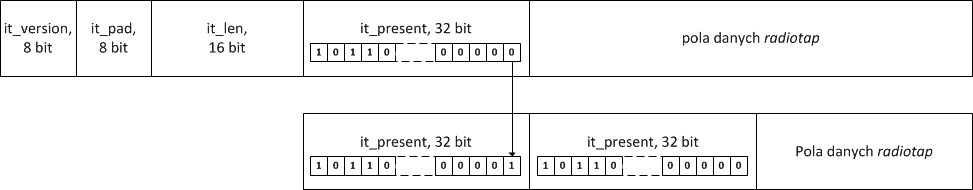
\includegraphics[width=325px]{img/RadiotapHeader}
\caption{Nagłówek \emph{radiotap}.}
\label{RadiotapHeader}
\end{center}
\end{figure}

Funkcja przetwarzająca aplikacji \emph{hop-sniffer} otrzymuje na wejściu ramkę w postaci ciągu bajtów. Ciąg ten zostaje rzutowany na strukturę odpowiadającą wyżej opisanemu składowi nagłówka i odczytywane jest pole \emph{it\_len}. Odczytywanie danych z nagłówka wymaga ekstrakcji z formatu \emph{little endian}, w którym są one kodowane. Parametr ten jest wykorzystywany do obliczenia wskaźnika na koniec nagłówka \emph{radiotap}.

Pierwszym krokiem jest odnalezienie ostatniej bitmapy \emph{it\_present} sprawdzając jej 31 bit i ewentualnie przesuwając wskaźnik o 32 kolejne. Za bitmapami znajdują się pola przechowujące dane w naturalnym porządku binarnym (co 8, 16, 32 itd. bitów). Są one rozmieszczane według tego samego porządku co odzwierciedlające je numery wewnątrz map \emph{it\_present}.

Następnie program pomiarowy przegląda dostępne bitmapy i dla każdego kolejnego, ustawionego bitu rozpakowuje odpowiadające mu pole danych. Przeglądanie bitmapy od najmniej znaczącego bitu polega na odjęciu od niej liczby 1 i wykonania operacji XOR między tablicą wynikową i wejściową. W ten sposób program otrzymuje bitmapę z ustawionym jedynie aktualnie najmniej znaczącym bitem. W celu określenia odpowiadającego mu pola \emph{radiotap} należy obliczyć na której pozycji w 32-bitowym słowie się on znajduje. Odnalezienie pozycji realizowane jest za pomocą zagnieżdżonego makra, które wykonuje przesunięcia bitowe w prawo sprawdzając czy otrzymane słowo równe jest zeru. Przesunięcia wykonywane są kolejno połowiąc pozostałe do sprawdzenia słowo, czyli kolejno o 16, 8, 4 i 2 bity. Jeśli przesunięcie wyzerowało tablicę oznacza to, że bit znajduje się na numerze pozycji mniejszym niż przesunięcie i należy ponownie wywołać makro dla tej samej tablicy przesuwając o połowę mniej bitów. Otrzymanie słowa niezerowego oznacza, że numer bitu jest wyższy niż przesunięcie. W tym przypadku można zwrócić sumę liczby przesuniętych bitów (szukany numer jest większy) i wywołania makra przesuwającego o dwukrotnie mniejszą ilość bitów, ale dla aktualnego (już przesuniętego) słowa. Jest to implementacja wzorowana na algorytmie wyszukiwania binarnego opartego na idei \emph{dziel i zwyciężaj} co sugeruje jej działanie w czasie logarytmicznym. 

Specyfikacja \emph{radiotap} zakłada, że programista znający nazwę pola zna również jego rozmiar. Pola danych rozmieszczone są zgodnie z naturalnym porządkiem binarnym. Oznacza to, że odczytując słowo określonej wielkości należy sprawdzić, czy mieści się ono w do tej pory przetworzonym fragmencie danych całkowitą liczbę razy. Jeśli tak nie jest to słowo należy odczytać z pozycji znajdującej się o brakującą liczbę bitów dalej, gdyż program trafił na wypełnienie (ang. \emph{padding}). Jest to przyjęty standard konstrukcji nagłówka \emph{radiotap}, więc \emph{hop-sniffer} również go respektuje. Przykładowo \ref{RadiotapUnpack}, jeśli do tej pory program odczytał trzy pola o rozmiarze 8 bitów i otrzymuje polecenie odczytania słowa 16-bitowego to powinno być ono odczytane z adresu (uznając początek przestrzeni danych za 0) 32, a nie 24. 

\begin{figure}[htb]
\begin{center}
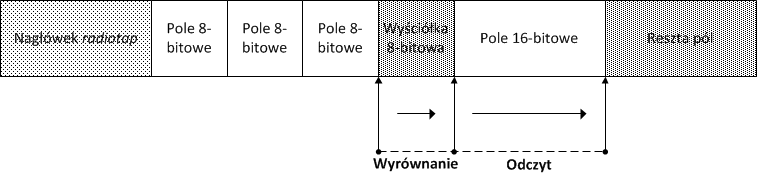
\includegraphics[width=378px]{img/RadiotapUnpack}
\caption{Wyrównanie do naturalnego porządku binarnego i rozpakowanie pola \emph{radiotap}.}
\label{RadiotapUnpack}
\end{center}
\end{figure}

Do rozpakowywania pól danych nagłówka \emph{radiotap} służy struktura \emph{unpacker} \ref{code:Unpacker}. Pole \emph{u\_buf} inicjowane jest przez adresem pierwszego bajtu za ostatnią bitmapą \emph{it\_present}, \emph{u\_next} za pomocą  wskaźnika na bajt za ostatnim odczytanym słowem, a \emph{u\_len} jest różnicą wskaźnika na początek ramki i ostatnią bitmapę. 

\lstset{caption={Struktura \emph{unpacker}.}, label={code:Unpacker}}
\begin{lstlisting}[frame=tb]
struct unpacker {
        /** 
         * Pointer to the beginning of 
         * radiotap data fields area of packet. 
         */
	u_int8_t *u_buf;
        /** 
         * Pointer to the next packet 
         * area that was not yet extracted. 
         */
	u_int8_t *u_next;
        /** 
         * Length of the radiotap data 
         * fields area. 
         */
	size_t u_len;
};
\end{lstlisting}

Po odczytaniu każdego słowa zgodnie z wyżej opisanymi regułami wskaźnik \emph{u\_next} przenoszony jest do przodu o jego długość. Wskaźnik na początek fragmentu danych służy do obliczania ewentualnych wypełnień (ang. \emph{padding}), a długość fragmentu do kontroli poprawności (jako warunek zatrzymujący przetwarzanie).

Odczytanie z bitmapy ustawionego bitu na pozycji 1 oznacza atrybut \emph{IEEE80211\_RADIOTAP\_FLAGS}, który zgodnie ze specyfikacją ma 8 bitów. Po rozpakowaniu jest on porównywany z maską \emph{0x10} (właściwość oznaczająca dodatkowy odstęp za nagłówkiem 802.11) i \emph{0x20} (ramka posiada fragment FCS). W pierwszym przypadku program ustawia zmienną \emph{pad} na wartość 1, w drugim zmienną \emph{fcslen} na wartość 4. Obydwie zmienne przekazywane są do procedury przetwarzania ramki standardu 802.11, gdzie będą potrzebne. 

Nagłówek \emph{radiotap} przechowuje również szczegółowe informacje dotyczące częstotliwości i mocy nadawania interfejsu przez, który został utworzony. Właściwość ta nie ma zastosowania w pomiarze roamingu 802.11, ale może być przydatna w bardziej skomplikowanych scenariuszach. Przetwarzanie nagłówka udostępnia więcej \emph{meta-danych} dotyczących kanału komunikacyjnego co stanowczo przemawia na jego korzyść. 

\subsection{Przetwarzanie nagłówka standardu \emph{802.11}.}

Wskaźnik \emph{packet} na początek migawki przechwyconej ramki \ref{RadiotapWifi} trafia na wejście funkcji przetwarzania nagłówka standardu 802.11 po przesunięciu o \emph{it\_len} bitów w przód. Tym samym powinien wskazywać na początek elementu FC (ang. \emph{Frame control}). Do funkcji przekazane zostają również wartości zmiennych \emph{pad} i \emph{fcslen} wyliczone w procesie przetwarzania nagłówka \emph{radiotap}. 

\begin{figure}[htb]
\begin{center}
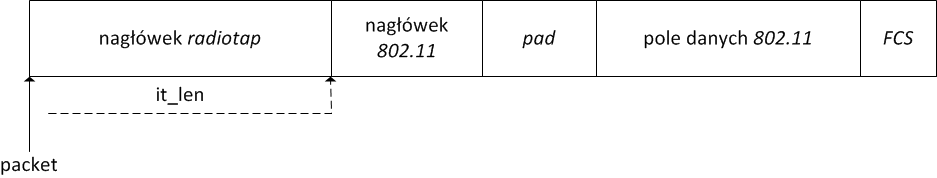
\includegraphics[width=312px]{img/RadiotapWifi}
\caption{Przesunięcie wskaźnika na początek ramki poza nagłówek \emph{radiotap}.}
\label{RadiotapWifi}
\end{center}
\end{figure}

Na podstawie danych uzyskanych z pakietu na tym etapie podejmowane są główne kroki procedury pomiarowej. Scenariusz pomiaru można rozumieć jako globalną strukturę, której pola wypełniane są w zależności od przepływu programu w wyniku wykrytego zdarzenia. Część struktur jest globalna, gdyż jest to bardziej wydajne niż przekazywanie ich bardzo głęboko w zagnieżdżonych wywołaniach funkcji, a taką właśnie strukturę ma program \emph{hop-sniffer}. 

Zgodnie z ustaleniami procedury pomiaru roamingu stacji klienckiej program powinien wykrywać dwa typy zdarzeń:
\begin{itemize}
\item[--] Odebranie ramki typu \emph{MGMT} i podtypu \emph{Association Response}.
\item[--] Odebranie ramki typu \emph{MGMT} i podtypu \emph{Disassociation}.
\end{itemize}
Sterują one przebiegiem obserwacji zjawiska, które posiada trzy zidentyfikowane stany:
\begin{enumerate}
\item Stan asocjacji z początkowym punktem dostępowym.
\item Stan przełączania kanału radiowego.
\item Stan asocjacji z docelowym punktem dostępowym.
\end{enumerate}
Stanom tym odpowiadają dobrze zdefiniowane zdarzenia. Odebranie ramki typu \emph{Association Response} z adresem źródłowym MAC początkowego punktu dostępowego wprowadza scenariusz pomiarowy w stan pierwszy. Sytuacja ta zmienia się po odebraniu ramki typu \emph{Disassociation} z adresem źródłowym MAC stacji klienckiej. Oznacza to, że stacja rozpoczęła proces roamingu i tym samym wprowadziła procedurę pomiarową w stan drugi. Ostatecznie pomiar kończy wejście scenariusza w stan trzeci spowodowane odebraniem ramki typu \emph{Association Response} z adresem źródłowym MAC docelowego punktu dostępowego, który potwierdza asocjację przybywającej stacji klienckiej.

Pierwszą czynnością jest ekstrakcja 16-bitowego pola FC (ang. \emph{Frame control}). Znajduje się ono na początku nagłówka, ale podczas rzutowania należy obsłużyć kodowanie \emph{litte endian}.

Aplikacja \emph{hop-sniffer} rozpoczyna przetwarzanie pola FC od ekstrakcji typu pakietu. W pomiarze roamingu 802.11 biorą udział jedynie ramki typu \emph{T\_MGMT}. Odczytanie typu odbywa się za pomocą makra. Wykonywane jest przesunięcie wskaźnika na pole FC poza znacznik protokołu, czyli o 2 bajty w lewo i zastosowanie do niego maski bitowej \emph{0x3}, która odczytuje 2 pierwsze bity ramki. Jeśli odczytane bity wynoszą \emph{0x0} (typ ramek MGMT) to program kontynuuje obsługę. Ramki nie będące typu \emph{T\_MGMT} są porzucane. 

Kolejnym krokiem jest rozgałęzienie przepływu programu na obsługę wybranych podtypów ramek \emph{MGMT}. Stosuję instrukcję warunkową \emph{switch} z argumentem będącym odczytanym podtypem ramki. Makro ekstrakcji podtypu dokonuje przesunięcia wskaźnika na pole FC o 4 bajty w lewo (pozbywa się znacznika protokołu i typu ramki) i stosuje maskę \emph{0xF}, która oznacza odczytanie ostatnich 4 bitów.

\begin{figure}[htb]
\begin{center}
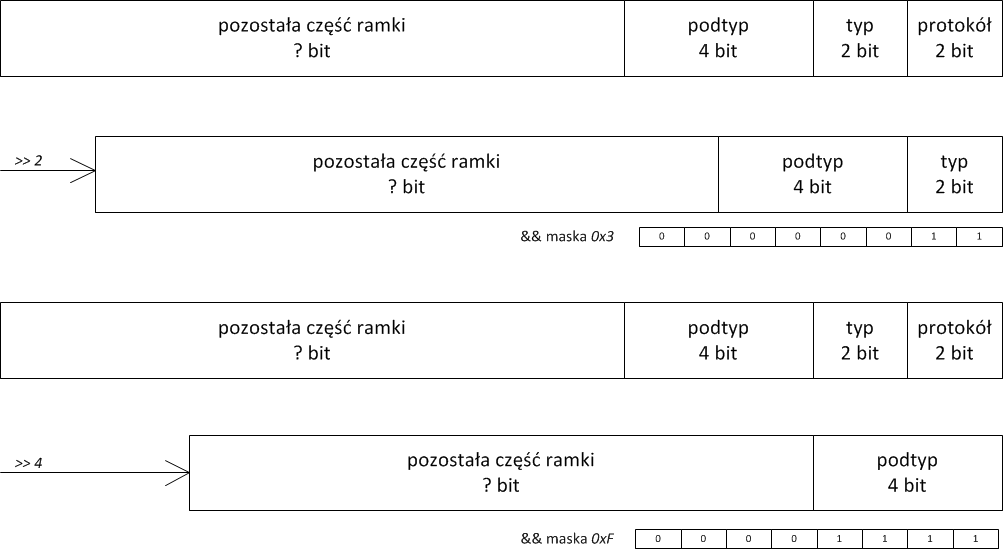
\includegraphics[width=333px]{img/TypeSubtype}
\caption{Ekstrakcja typu i podtypu z nagłówka \emph{802.11}.}
\label{TypeSubtype}
\end{center}
\end{figure}

Ostatnią brakującą daną jest adres źródłowy MAC obsługiwanego pakietu. Najłatwiej dostać się do tej informacji poprzez rzutowanie otrzymanego w argumentach wywołania funkcji wskaźnika na początek nagłówka standardu 802.11 typu \emph{MGMT} na jego reprezentację w postaci struktury danych języka \emph{C} \ref{code:MgmtHeader}. Krok ten ułatwia dostęp do dwóch 6-bajtowych tablic \emph{sa} i \emph{da} odpowiadających źródłowemu i docelowemu adresowi MAC ramki. Pozostałe pola są zgodne ze specyfikacją i odpowiadają kolejno polu kontrolnemu, polu \emph{duration} odpowiadającemu pozostałemu czasowi z tablicy \emph{NAV}, polu \emph{BSSID} (ang. \emph{Basic Service Set Identifier}) i numerowi kontrolnemu sekwencji.

\lstset{caption={Struktura \emph{mgmt\_hdr}.}, label={code:MgmtHeader}}
\begin{lstlisting}[frame=tb]
struct mgmt_hdr
{
        u_int16_t fc;
        u_int16_t duration;
        u_int8_t da[6];
        u_int8_t sa[6];
        u_int8_t bssid[6];
        u_int16_t seq_ctrl;
};
\end{lstlisting}



\subsection{Przełączanie kanału radiowego stacji pomiarowej.}

Podstawową charakterystyką interfejsu karty radiowej jest jego praca wyłącznie na jednej częstotliwości w danej chwili. Popularne programy przechwytywania ramek komunikacji bezprzewodowej (np. \emph{Wireshark}) udostępniają opcję ciągłej zmiany kanału pracy w celu obrazowania ruchu w całym spektrum dostępnym w medium transmisyjnym (ang. \emph{channel hopping}). Z punktu widzenia aplikacji \emph{hop-sniffer} zachowanie takie utrudniałoby i wprowadzało zakłamania kalkulacji opóźnień wybranych zjawisk. Nie zmienia to faktu, że w obserwacji przełączania częstotliwości pracy podczas roamingu 802.11 potrzebna jest jednorazowa zmiana kanału interfejsu urządzenia przechwytującego.     

Jednym z możliwych rozwiązań, które wyklucza potrzebę przełączania kanału jest użycie dwóch kart radiowych pracujących odpowiednio na częstotliwości każdego z punktów dostępowych biorących udział w eksperymencie. Ideą programu \emph{hop-sniffer} jest jednak możliwość uruchomienia na niewielkim komputerze przenośnym i łatwa implementacja procedur pomiarowych w oparciu o pojedynczy interfejs przechwytujący. 
Zastosowane rozwiązanie jest zgodne z założeniem o przeprowadzaniu scenariusza pomiarowego w odpowiedzi na wykryte zdarzenia (ramki protokołu) i wykorzystuje metodę jawnego przełączenia kanału pracy karty radiowej. Zastosowałem udostępniany przez sterownik interfejs wywołań systemowych IOCTL, za pomocą którego program nasłuchujący wystosowuje polecenie SIOCSIWFREQ służące do wprowadzenia urządzenia w podaną w jednostkach hertz częstotliwość pracy. 

Procedurę można podzielić na następujące fazy:
\begin{enumerate}
\item Otwarcie gniazda, które umożliwi wywołanie polecenia.
\item Przygotowanie argumentów wywołania w postaci akceptowanej przez polecenie.
\item Wywołanie IOCTL SIOCSIWFREQ w odpowiedzi na przetworzenie ramki typu \emph{Disassociation}.
\end{enumerate}

Program dąży do otwarcia gniazda AF\_INET (ang. \emph{Internet socket}) dostępnego na systemach Linux. Przewidziana jest też możliwość rozwoju i przyszłej przenośności aplikacji w postaci prób stworzenia innych użytecznych gniazd (IPX, AX.25, APPLETALK) w wypadku niedostępności gniazda typu \emph{Berkeley socket}. Otwarcie następuje z parametrem SOCK\_DGRAM niezbędnym do wywołania typu IOCTL.

Argumentem wywołania jest struktura \emph{iwreq} będąca zmodyfikowaną wersją \emph{ifreq} posiadającą dodatkowe elementy unii \emph{u} w tym pole \emph{freq}. Jest to pole typu \emph{iw\_freq} rozdzielające wartość częstotliwości (daną w postaci zmiennoprzecinkowej) na mantysę i wykładnik, gdyż jądro nie udostępnia arytmetyki zmiennoprzecinkowej.

% Wzory na ekstrakcję m i e!

Jeśli podczas przetwarzania wykryta zostanie ramka typu \emph{Disassociation} to program \emph{hop-sniffer} przełącza kanał interfejsu nasłuchującego na częstotliwość nowego punktu dostępowego w celu przechwycenia stempla czasowego momentu asocjacji stacji klienckiej i tym samym zakończenia roamingu 802.11.


\begin{figure}[htb]
\begin{center}
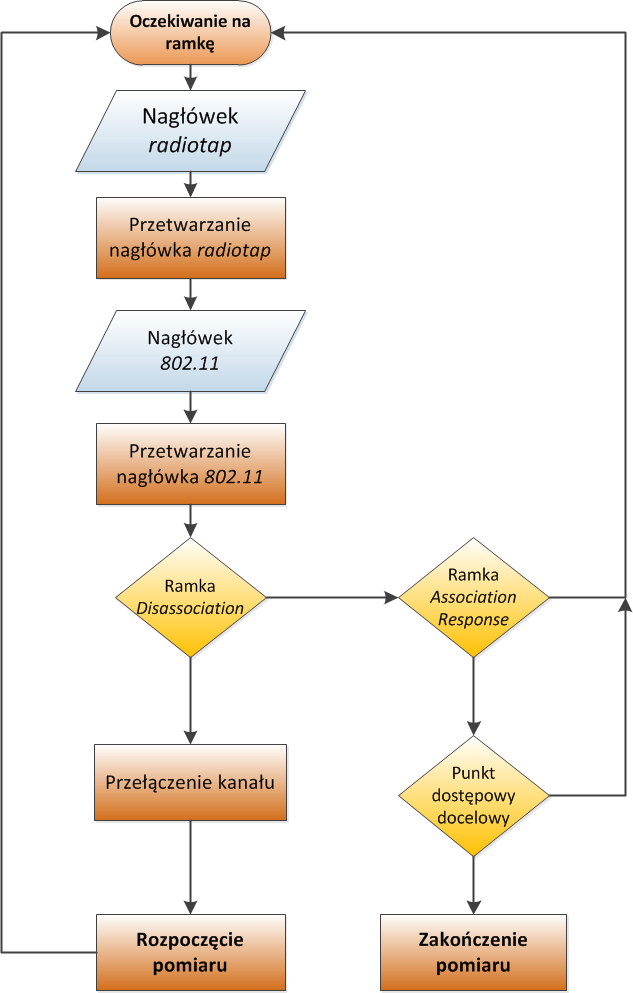
\includegraphics[width=210px]{img/FlowDiagram}
\caption{Diagram przepływu sterowania programu \emph{hop-sniffer}.}
\label{FlowDiagram}
\end{center}
\end{figure}

























\chapter{Wnioski z pomiaru roamingu \emph{802.11}.}
%


\chapter{Kierunki rozwoju.}
% Podsumowanie

Głównym celem było stworzenie narzędzia otwartego na rozwój. Skuteczne przeprowadzenie obserwacji opisywanego zjawiska dowodzi użyteczności zastosowanego podejścia. Ostatecznie implementacji uległa część dotycząca roamingu, ale program oferuje bazę do wdrożenia innych procedur pomiarowych, pod warunkiem, że ich elementarnymi krokami są zdarzenia przesłania ramek standardu 802.11. Uniwersalność rozwiązania może zostać zwiększona dzięki zastosowaniu interfejsu użytkownika do komponowania niezdefiniowanych scenariuszy. Cel ten może zostać łatwo osiągnięty przez wprowadzenie dodatkowej abstrakcji procedury pomiarowej, która sprowadza się do określenia różnicy stempli czasowych wybranych zdarzeń (określanych przez typy ramek i ich zawartość).

Aplikacja ukazuje sposób podejścia do potrzeby przełączania kanału radiowego w trakcie realizacji scenariusza bez groźby zgubienia ramek potrzebnych do jego kontynuacji. Bardziej efektywnym podejściem byłby wykorzystanie dwóch lub więcej interfejsów radiowych pracujących na różnych częstotliwościach. Wymaganie to można spełnić stosując dostępną w bibliotece \emph{libpcap} możliwość nasłuchiwania na wszystkich dostępnych interfejsach. Wymagałoby to uprzedniego wprowadzenia wybranych interfejsów \emph{monitor} w tryb \emph{promiscuous}, a następnie inicjalizacji nasłuchiwania przy pomocy nazwy interfejsu \emph{any}. Zbędny ruch można odrzucić za pomocą zaimplementowanego już mechanizmu filtra. Rozwiązanie to jest najprostsze i nie wymaga zmian w logice działania aplikacji (kolejności i metodzie przetwarzania pakietu).

Warto zaznaczyć, że program implementowany był z myślą o rozwoju w bardziej złożoną aplikację pomiarową. Z pewnością przydatne byłoby wprowadzenie wszelkich ułatwień dla użytkownika w postaci zwiększenia automatyzacji pomiaru z jednoczesną możliwością określenia sposobu prezentacji wyników oraz łatwy sposób definiowania scenariusza pomiarowego (za pomocą typów ramek i tekstu filtra).

W wyniku działania, w warunkach domowych, program uzyskał ciekawe wyniki. Część scenariuszy sugeruje, że przeprowadzenie pomiaru w warunkach izolowanych od wpływu środowiska zewnętrznego mogłoby pomóc w zebraniu danych wolnych od wartości odstających. Izolacja pozwoliłaby również na bardziej dokładną identyfikację czynników wpływających na zwiększanie opóźnienia roamingu.





\nocite{*}
\bibliography{bibliografia}
\end{document}
